\documentclass[10pt,twocolumn,a4paper]{article}
\usepackage[T1]{fontenc}
\usepackage[utf8]{inputenc}
\usepackage{times}
\usepackage{amsmath,amssymb}
\usepackage{graphicx}
\usepackage{booktabs}
\usepackage{array}
\usepackage{multirow}
\usepackage{xcolor}
\usepackage{microtype}
\usepackage[authoryear,round]{natbib}
\usepackage[hidelinks]{hyperref}
\usepackage[font=small,labelfont=bf,labelsep=period]{caption}
\usepackage[a4paper,top=2.0cm,bottom=2.0cm,left=1.7cm,right=1.7cm,columnsep=0.62cm]{geometry}
\usepackage{fancyhdr}
\usepackage{titlesec}

\definecolor{elsblue}{RGB}{0,86,150}
\hypersetup{colorlinks=true,linkcolor=elsblue,citecolor=elsblue,urlcolor=elsblue}

\titleformat{\section}{\normalfont\bfseries\fontsize{10}{12}\selectfont}{\thesection.}{0.5em}{}
\titleformat{\subsection}{\normalfont\itshape\fontsize{10}{12}\selectfont}{\thesubsection.}{0.5em}{}
\titlespacing*{\section}{0pt}{10pt}{5pt}
\titlespacing*{\subsection}{0pt}{8pt}{4pt}

\pagestyle{fancy}
\fancyhf{}
\fancyhead[L]{\footnotesize\itshape Reproduction Study}
\fancyhead[R]{\footnotesize\itshape Ecological Informatics --- Reproduction of 85 (2025) 102961}
\fancyfoot[C]{\footnotesize\thepage}
\renewcommand{\headrulewidth}{0.3pt}

\setlength{\parindent}{1.2em}
\setlength{\abovecaptionskip}{4pt}
\setlength{\belowcaptionskip}{2pt}
\renewcommand{\arraystretch}{1.12}

\newcommand{\evc}[1]{{\footnotesize\texttt{#1}}}

\begin{document}

\long\def\FrontMatterBlock{%
\vspace{-0.6cm}
{\footnotesize\color{elsblue} Reproduction and audit of \emph{Ecological Informatics} 85 (2025) 102961\par}
\vspace{2pt}
\noindent\rule{\textwidth}{0.6pt}
\vspace{10pt}

{\fontsize{17}{20}\selectfont An independent reproduction and reproducibility audit of multilayer
perceptron models for mangrove species identification from Sentinel-2 multispectral data\par}

\vspace{10pt}
{\fontsize{11}{13}\selectfont Bala Sudalaimuthu\,$^{a,*}$\par}
\vspace{4pt}
{\footnotesize\itshape $^{a}$ [Artificial Intelligence and Machine, Thakur College of Engineering and Technology, Mumbai, India]\par}

\vspace{12pt}
\noindent\rule{\textwidth}{0.4pt}
\vspace{6pt}

\noindent
\begin{minipage}[t]{0.23\textwidth}
\footnotesize
\textbf{A R T I C L E \ \ I N F O}\par\vspace{6pt}
\textit{Keywords:}\par
Reproducibility\par
Mangrove species mapping\par
Multilayer perceptron\par
Sentinel-2\par
Spectral separability\par
Threats to validity\par
Data availability audit
\end{minipage}
\hfill
\begin{minipage}[t]{0.72\textwidth}
\footnotesize
\textbf{A B S T R A C T}\par\vspace{6pt}
Independent reproduction is a necessary complement to the rapid adoption of deep learning in
ecological remote sensing. This study reports an evidence-classified independent reproduction and
reproducibility audit of Monterrubio-Mart\'inez et al. (2025), who trained multilayer perceptron
(MLP) models on Sentinel-2 multispectral reflectance to map monospecific mangrove forests of
\emph{Rhizophora mangle}, \emph{Avicennia germinans} and \emph{Laguncularia racemosa} in La Mancha,
Veracruz, Mexico. This study is not intended to invalidate the original work; its purpose is to
determine, element by element, which parts of the original methodology can be independently
verified from the artefacts the original authors made publicly available and which cannot. Every
methodological element was classified as \evc{PAPER-SPECIFIED}, \evc{DATA-DERIVED},
\evc{IMPLEMENTATION ASSUMPTION}, \evc{DATA-LIMITED} or \evc{NOT AVAILABLE} across a 33-point
specification matrix and a dedicated reproducibility audit table. The public repository
(1{,}605{,}681 pixels, 147 cloud-free Sentinel-2 L1C acquisitions, 2015--2021) was audited, and the
exploratory statistical analysis of the original work was reproduced from the released data:
one-way ANOVA on each of the ten spectral bands and all thirty pairwise Tukey HSD comparisons
returned significant species differences ($p<0.05$), consistent with the published Fig.~4. The
architectural grid of the original study (a logistic baseline plus five hidden-layer depths
$\times$ eight layer widths, 41 configurations) was re-implemented and trained, under a stratified
random pixel-level holdout, on a class-balanced 30{,}000-pixel three-species dataset drawn from the
released file; this reproduction therefore evaluates three-class mangrove-species discrimination
and cannot reproduce the original binary mangrove/non-mangrove task or the original four-class
task, because the non-mangrove pixels are not part of the public deposit. Test accuracy under this
holdout ranged from 69.64\,\% for the logistic baseline to 94.98\,\% for the four-layer,
300-neuron model; the architecture identified by the original authors as the most reliable for
spatial mapping (five layers, 50 neurons) attained 90.22\,\% test accuracy with a smaller
train--test gap (2.14 percentage points) than wider architectures of comparable depth (4.4--4.7
percentage points), a pattern consistent with the hypothesis that restricting layer width may limit
overfitting in this setting. The binary 60{,}000-pixel and four-class 40{,}000-pixel experiments,
and the full-scene raster predictions of Figs.~7--10, could not be reproduced numerically because
the non-mangrove background pixels, the UAV orthophoto and the Sentinel-2 scene GeoTIFFs were not
deposited. Reported accuracies are therefore treated throughout as reference benchmarks rather than
reproduction targets, no superiority claim is made in either direction, and a dedicated threats-to-
validity analysis discusses the internal, statistical, external and reproducibility-related
limitations of both the original study and this audit. All reproduction code, notebooks and
generated results are released publicly.
\end{minipage}

\vspace{8pt}
\noindent\rule{\textwidth}{0.4pt}
\vspace{14pt}
}

\twocolumn[\begin{@twocolumnfalse}\FrontMatterBlock\end{@twocolumnfalse}]


\renewcommand{\thefootnote}{}
\footnotetext{$^{*}$ Corresponding author. E-mail address: bala010706@gmail.com}
\renewcommand{\thefootnote}{\arabic{footnote}}

\section{Introduction}
\label{sec:intro}

Mangroves are evergreen forests of tropical and subtropical intertidal environments whose
composition varies with the presence, abundance and dominance of species, so that stands are
classified as monospecific when one species predominates or as mixed when several species occur
together with other wetland vegetation \citep{fao2023}. Their global extent has contracted
markedly since the beginning of the century as a consequence of land-use change for livestock,
aquaculture, urbanisation and tourism \citep{morenocasasola2002}, and the resulting demand for
low-cost, repeatable monitoring has made open-access satellite constellations such as Sentinel-2
the instrument of choice for regional mangrove mapping \citep{chopade2023,pham2019}.

Within this setting, \citet{monterrubio2025} presented an approach that integrates unmanned aerial
vehicle (UAV) photogrammetry with Sentinel-2 multispectral reflectance to train multilayer
perceptron (MLP) models capable of mapping both mixed and monospecific mangrove forests at the
species level in Veracruz, Mexico. Their best binary models reached accuracies of 99.95\,\% for
training and 99.8\,\% for test, while at the species level the best multiclass models attained
98.73\,\% for training and 96.84\,\% for test. Crucially, the authors also demonstrated that the
highest tabular accuracy did not necessarily yield the most reliable spatial distribution, and
selected a comparatively modest five-hidden-layer, 50-neuron architecture as the most trustworthy
model for real-world mapping. That observation --- that accuracy and spatial fidelity can diverge
--- is the kind of claim that independent reproduction is best placed to test.

Reproducibility, however, remains unevenly practised in ecological informatics. A published
accuracy figure is only interpretable when the dataset partition, the class definitions, the
optimisation hyperparameters and the random seeds that produced it are recoverable. Where those
elements are absent, a numerical mismatch between an original study and its reproduction carries no
information about either implementation, because the two experiments are not testing the same
hypothesis. The purpose of the present study is therefore not to re-derive the published numbers,
nor to compete with them, but to establish precisely which claims of \citet{monterrubio2025} can be
independently verified from the artefacts the authors deposited, which cannot, and why.

Three research questions organise the work. First, can the exploratory and statistical analysis of
the original study --- the demonstration that the three mangrove species differ significantly in
every Sentinel-2 band --- be reproduced from the released data? Second, can the capacity-related
generalisation pattern reported by the authors, in which a comparatively narrow deep network was
judged more reliable for spatial mapping than higher-accuracy alternatives, be examined on the data
that is publicly available? Third, which components of the original pipeline are irrecoverable from
the public record, and what is the appropriate scientific language for reporting results obtained
on a dataset that differs in class space from the one the authors used?

To answer these questions every parameter of the original methodology was assigned to one of five
evidence classes, the complete 41-model architectural grid was re-implemented, and all comparisons
between reported and reproduced values are stated in percentage points with an explicit statement
of comparability. Consistent with the integrity constraints adopted here, no substitute or proxy
imagery was downloaded to stand in for the authors' unreleased rasters, no missing mask was
synthesised, and no non-mangrove samples were invented to force the original binary or four-class
experiments to run. This study does not seek to invalidate, replace or outperform the original
work; its scope is limited to determining which of its claims are independently verifiable from
the publicly recoverable evidence, and under what conditions.

The contribution of this work is accordingly methodological rather than purely empirical. It
offers (i) an explicit five-label evidence taxonomy for auditing reproducibility claims in
ecological deep learning studies; (ii) a file-by-file audit of which data and methodological
artefacts of \citet{monterrubio2025} are publicly recoverable and which are not; (iii) an
independent reproduction of the original exploratory statistical analysis on the released data;
(iv) an independent re-implementation of the full 41-configuration MLP grid on the reproducible
three-class subset of that data; (v) an analysis of model capacity and train--test gap across that
grid, examined as a quantitative complement to the original authors' qualitative spatial
argument; (vi) an explicit identification of the artefacts that prevent reproduction of the
original binary, four-class and spatial experiments; and (vii) a threats-to-validity analysis that
makes the boundary between reproducible and non-reproducible components, and between statistical
significance and practical separability, explicit for the reader.

\section{Material and methods}
\label{sec:methods}

Fig.~\ref{fig:boxplots} onwards summarise the analytical chain followed in this reproduction. The
chain mirrors the four stages of the original study --- data acquisition, exploratory and
statistical analysis, deep learning models, and model test --- but adds an explicit auditing stage
in which each stage is annotated with the evidence available to support it.

\subsection{Evidence classification taxonomy}
\label{sec:taxonomy}

Because a reproduction must distinguish what a paper states from what a reproducer assumes, every
methodological element was assigned one of five labels. \evc{PAPER-SPECIFIED} denotes an element
stated explicitly in the text, tables, figures or equations of \citet{monterrubio2025}.
\evc{DATA-DERIVED} denotes an element computed directly from the authors' deposited dataset or its
metadata. \evc{IMPLEMENTATION ASSUMPTION} denotes an element absent from the paper and chosen here
on the basis of standard practice, always documented. \evc{DATA-LIMITED} denotes an element
described in the paper but omitted from the public deposit. \evc{NOT AVAILABLE} denotes an element
absent from both the text and the released artefacts. Table~\ref{tab:spec} reports the resulting
classification for the principal elements of the pipeline.

\subsection{Data acquisition and availability audit}
\label{sec:dataaudit}

The original study collected field data on species distribution at two sites in Veracruz, Mexico:
La Mancha ($19^{\circ}35'12''$\,N, $96^{\circ}23'09''$\,W), a priority conservation site with a
9{,}050\,km$^2$ region of influence chosen for its well-defined monospecific stands, and Arroyo
Moreno ($19^{\circ}00'59''$\,N, $96^{\circ}03'43''$\,W), used as an independent site to test
scalability \evc{PAPER-SPECIFIED}. A DJI Mavic Mini 2 UAV acquired 5{,}435 zenithal photographs at
100\,m altitude in July 2021, processed in Agisoft Metashape Professional v1.8.5 into a 3.5\,cm
orthophoto, and 100 ground control points were surveyed with a Garmin GPSMAP 527 by walking and
boat transects. Monospecific polygons for red (\emph{R.\ mangle}), black (\emph{A.\ germinans}) and
white (\emph{L.\ racemosa}) mangrove, together with mixed mangrove and flooded freshwater forested
wetland, were digitised in QGIS v3.22.14.

A total of 147 cloud-free Sentinel-2 L1C acquisitions spanning 2015--2021 were obtained from the
Copernicus Browser, converted to surface reflectance, and the 20\,m red-edge and shortwave infrared
bands (B5, B6, B7, B8A, B11, B12) were resampled bilinearly with \texttt{rasterio} in Python 3.8.13
to the 10\,m grid of B2, B3, B4 and B8. Ten bands entered the models: B2 (490\,nm), B3 (560\,nm),
B4 (665\,nm), B5 (705\,nm), B6 (740\,nm), B7 (783\,nm), B8 (842\,nm), B8A (865\,nm), B11
(1610\,nm) and B12 (2190\,nm); the coastal aerosol, water vapour and cirrus bands were excluded.
Features were standardised with the scikit-learn 1.2.1 \texttt{StandardScaler}, $z=(x-\mu)/\sigma$.
No vegetation index was computed, the authors having argued that reflectance in its purest form is
preferable to derived indices for model training.

The deposited repository was then audited file by file. Two artefacts are present:
\texttt{DataBase\_Sentinel\_2\_Mangrove\_LaMancha.csv} (191\,MB; 1{,}605{,}681 rows $\times$ 12
columns) and an Ecological Metadata Language v2.2.0 XML descriptor \evc{DATA-DERIVED}. The row
count is internally consistent with the stated acquisition design: 10{,}923 labelled pixels per
scene across 147 scenes, distributed as 9{,}806 \emph{A.\ germinans}, 856 \emph{R.\ mangle} and 261
\emph{L.\ racemosa} per scene, giving totals of 1{,}441{,}482 (89.77\,\%), 125{,}832 (7.84\,\%) and
38{,}367 (2.39\,\%) pixels respectively.

Four categories of artefact described in the paper are absent from the deposit
\evc{DATA-LIMITED}: the non-mangrove background reflectance table; the subsampled 60{,}000-row
binary and 40{,}000-row four-class datasets; the UAV orthophoto GeoTIFF and QGIS vector masks; and
the Sentinel-2 scene GeoTIFFs for La Mancha and Arroyo Moreno on which Figs.~7--10 of the original
article were produced. The consequence is structural rather than incidental: the binary and
four-class experiments of the original study cannot be reconstructed, because three of the four
classes in the multiclass problem and one of the two classes in the binary problem are unavailable.

\subsection{Exploratory and statistical analysis}
\label{sec:methods-stats}

Following the original protocol, a one-way analysis of variance was performed independently on each
of the ten bands to test whether mean reflectance differs among the three species, followed by a
Tukey honestly significant difference post-hoc test at a 95\,\% confidence interval ($\alpha=0.05$)
for the three pairwise contrasts \emph{A.\ germinans} vs \emph{R.\ mangle}, \emph{A.\ germinans} vs
\emph{L.\ racemosa} and \emph{R.\ mangle} vs \emph{L.\ racemosa} \evc{PAPER-SPECIFIED}. The original
study used the \texttt{bioinfokit} v1 package; the present reproduction used equivalent
implementations in the SciPy and statsmodels stack, a substitution that does not alter the
test statistics. Mean reflectance curves with one standard deviation envelopes, kernel density
estimates for the most diagnostic bands, and the Pearson correlation matrix of the ten bands were
computed in addition, to characterise the structure of the feature space that the classifiers
operate on.

\subsection{Multilayer perceptron models}
\label{sec:methods-mlp}

The model family was re-implemented following the architectural specification given in the
original text. The baseline is a single
input-to-output layer, interpretable as a logistic regression; the MLPs comprise one to five hidden
layers, each evaluated at eight widths (5, 10, 20, 50, 100, 150, 300 and 500 neurons), giving
$1+5\times8=41$ configurations per task \evc{PAPER-SPECIFIED}. All hidden layers use ReLU
activations. The binary task uses a sigmoid output with binary cross-entropy,
\begin{equation}
\mathcal{L}_{\mathrm{BCE}}=-\frac{1}{N}\sum_{i}\left[y_i\log\hat{y}_i+(1-y_i)\log(1-\hat{y}_i)\right],
\end{equation}
and the multiclass task a softmax output with categorical cross-entropy,
\begin{equation}
\mathcal{L}_{\mathrm{CCE}}=-\frac{1}{N}\sum_{i}\sum_{k}y_{i,k}\log\hat{y}_{i,k}.
\end{equation}
Adam is the optimiser in both cases. Data were split 70\,\% for training and 30\,\% for testing
with \texttt{train\_test\_split}.

Four optimisation settings are \evc{NOT AVAILABLE} in the original text and were fixed here as
documented \evc{IMPLEMENTATION ASSUMPTION}, applied identically across the full grid: learning rate
$\alpha=0.001$ (the Adam default, with $\beta_1=0.9$, $\beta_2=0.999$, $\epsilon=10^{-8}$), batch
size 256, and 30 training epochs with full loss tracking to verify convergence. A single fixed seed
(42) was used uniformly for every stochastic step of the reproduction pipeline: NumPy random state,
PyTorch CPU and, where applicable, GPU/MPS weight initialisation, the pandas sampling calls that
drew the balanced 10{,}000-per-species subset, and the \texttt{scikit-learn}
\texttt{train\_test\_split} call. Because these values are not reported by
\citet{monterrubio2025}, they remain \evc{IMPLEMENTATION ASSUMPTION} relative to the original
study even though they are fully documented and fixed within this reproduction; only a single seed
was run, so no multi-seed variance estimate is available
[AUTHOR INPUT REQUIRED: multi-seed replicate runs, if executed, would allow the stability of the
reported accuracies and train--test gaps to be quantified; none were performed for this version of
the manuscript]. The original work cites \citet{chollet2021}, indicating a Keras/TensorFlow
implementation; this reproduction uses PyTorch 2.8.0 under Python 3.9.6 on Apple Silicon (Metal
Performance Shaders backend), with scikit-learn 1.6.1, SciPy 1.13.1, statsmodels 0.14.6, pandas
2.3.3 and NumPy 2.0.2, as against the paper's stated Python 3.8.13 and scikit-learn 1.2.1. PyTorch's
default Kaiming-uniform initialisation for ReLU linear layers differs from the Glorot-uniform
default of Keras. Exact bit-level reproduction is therefore not achievable from the information
available, and only architectural trends and relative rankings are compared between the two studies.

Standardisation was implemented so as to avoid train--test contamination: the \texttt{StandardScaler}
was fit exclusively on the training partition and then used to transform both the training and test
partitions, rather than being fit on the full dataset before splitting. The original text (Section
2.2 of \citealp{monterrubio2025}) specifies the standardisation formula and the scikit-learn version
used but does not state the order in which scaling and splitting were performed; the paper's own
practice is accordingly \evc{NOT AVAILABLE} on this specific point, while the fit-on-train
procedure followed in this reproduction is stated here as a documented methodological choice,
consistent with standard practice for preventing data leakage, rather than as a fact established
about the original implementation.

Because the non-mangrove class was not deposited, the experiment executed here is a three-class
monospecific problem \evc{DATA-DERIVED}: 30{,}000 pixels balanced at 10{,}000 per species, split
21{,}000 for training (7{,}000 per species) and 9{,}000 for testing (3{,}000 per species) by
stratified random sampling at the pixel level (\texttt{stratify=y}). Per-class representation is
thus identical to the original 40{,}000-pixel design (10{,}000 per class); the number of classes,
and hence the chance baseline (33.3\,\% here against 25\,\% in the original four-class task),
differs. Because the released CSV pools pixels drawn from 147 Sentinel-2 acquisitions of the same
two study sites, and the split described above is performed at the pixel level without blocking by
scene or acquisition date, the same or a spatially adjacent ground location, imaged on a different
date, may appear in both the training and the test partition. The accuracy figures reported below
should accordingly be read as performance under a stratified random pixel-level holdout on this
specific multi-temporal stack, and not as evidence of generalisation to unseen geographic locations
or acquisition dates; this risk is examined further in the threats-to-validity analysis
(Section~\ref{sec:threats}) as an unverified structural limitation, since the available metadata do
not permit spatial blocking to be tested against the unblocked split reported here. Evaluation used
overall accuracy on both partitions, per-class precision, recall and $F_1$, confusion matrices, the
train--test gap
\begin{equation}
\Delta = \mathrm{Acc}_{\mathrm{train}}-\mathrm{Acc}_{\mathrm{test}},
\end{equation}
and total parameter count as a proxy for model capacity.

\subsection{Models test}
\label{sec:methods-modelstest}

The original spatial evaluation applied the trained models pixel-by-pixel to full Sentinel-2 scenes
over La Mancha and Arroyo Moreno and compared the predicted maps visually against the UAV
orthophoto ground truth. Since the scene GeoTIFFs, the orthophoto and the vector masks were not
deposited, this stage was conducted here as a documented audit rather than as a raster
reproduction. In keeping with the integrity rules adopted for this study, no unrelated satellite
imagery was substituted for the authors' scenes and no spatial mask was fabricated; instead, the
spatial claims of the original work were restated, and the spectral evidence bearing on them was
examined in the feature space that is available.

\begin{table*}[!t]
\centering
\caption{Evidence classification of the principal methodological elements of
\citet{monterrubio2025}, following the five-label taxonomy adopted in this reproduction.}
\label{tab:spec}
\footnotesize
\begin{tabular}{p{4.1cm} p{8.4cm} p{4.0cm}}
\toprule
\textbf{Element} & \textbf{Value in the original study} & \textbf{Classification} \\
\midrule
Study sites & La Mancha and Arroyo Moreno, Veracruz, Mexico & \evc{PAPER-SPECIFIED} \\
Sensor & Sentinel-2 MSI L1C, 147 cloud-free scenes, 2015--2021 & \evc{PAPER-SPECIFIED} \\
UAV photogrammetry & DJI Mavic Mini 2, 100\,m, 5{,}435 photos, 3.5\,cm orthophoto & \evc{PAPER-SPECIFIED} \\
Spectral bands & B2, B3, B4, B5, B6, B7, B8, B8A, B11, B12 (10 bands) & \evc{PAPER-SPECIFIED} \\
Resampling & Bilinear to 10\,m, \texttt{rasterio}, Python 3.8.13 & \evc{PAPER-SPECIFIED} \\
Standardisation & scikit-learn 1.2.1 \texttt{StandardScaler} & \evc{PAPER-SPECIFIED} \\
Released CSV & 1{,}605{,}681 rows; 10{,}923 pixels $\times$ 147 scenes & \evc{DATA-DERIVED} \\
Released class inventory & \emph{A.\ germinans} 1{,}441{,}482; \emph{R.\ mangle} 125{,}832; \emph{L.\ racemosa} 38{,}367 & \evc{DATA-DERIVED} \\
Binary dataset (60{,}000 px) & 30{,}000 mangrove + 30{,}000 non-mangrove & \evc{PAPER-SPECIFIED} / \evc{DATA-LIMITED} \\
Four-class dataset (40{,}000 px) & 10{,}000 px per class including non-mangrove & \evc{PAPER-SPECIFIED} / \evc{DATA-LIMITED} \\
Architecture grid & logistic $+$ 1--5 hidden layers $\times$ \{5,10,20,50,100,150,300,500\} & \evc{PAPER-SPECIFIED} \\
Activations, losses, optimiser & ReLU; sigmoid/BCE and softmax/CCE; Adam & \evc{PAPER-SPECIFIED} \\
Train/test split & 70\,\% / 30\,\%, \texttt{train\_test\_split} & \evc{PAPER-SPECIFIED} \\
Learning rate, batch size, epochs & not reported & \evc{NOT AVAILABLE} / \evc{IMPLEMENTATION ASSUMPTION} \\
Random seeds, initialisation & not reported & \evc{NOT AVAILABLE} / \evc{IMPLEMENTATION ASSUMPTION} \\
Scene GeoTIFFs, orthophoto, masks & used for Figs.~7--10 & \evc{DATA-LIMITED} \\
\bottomrule
\end{tabular}
\end{table*}

\section{Results}
\label{sec:results}

The results of this reproduction are presented below in the order of the original article: first
the exploratory and statistical analysis, then the multilayer perceptron models, and finally the
models test.

\subsection{Exploratory and statistical analysis}
\label{sec:results-stats}

Fig.~\ref{fig:boxplots} shows the reproduced boxplots for each band and species. The one-way ANOVA
and Tukey post-hoc test reveal a significant statistical difference between the species in all the
cases ($p<0.05$); across the ten bands every $F$-test returned $p<10^{-10}$ and all thirty pairwise
contrasts returned $p<0.001$. This is consistent, in its qualitative and inferential content, with
Fig.~4 of \citet{monterrubio2025} and indicates that there are detectable differences in the
spectral responses of each species. The pixel counts entering these tests are very large
(hundreds of thousands to over a million pixels per species), and with such sample sizes even
small, ecologically minor differences in mean reflectance will register as statistically
significant; the $p$-values reported here, like those of the original study, should therefore be
read as evidence that the three species are statistically distinguishable in this dataset, not as
a direct measure of how large or ecologically important the underlying differences are. Because the
pixels are not independent observations --- they are drawn repeatedly from the same monospecific
polygons across 147 temporally correlated acquisitions of the same two sites --- the classical ANOVA
assumption of independent samples is not strictly satisfied, and the test is best interpreted as a
faithful pixel-level reproduction of the original analysis rather than as an independent-site
statistical inference; this point is developed further in Section~\ref{sec:threats}.
[AUTHOR INPUT REQUIRED: standardised effect-size statistics (e.g. eta-squared or Cohen's $d$ per
band) and confidence intervals were not computed in the executed reproduction; if available in the
underlying analysis code they would allow the magnitude of the differences, and not only their
significance, to be reported alongside Fig.~\ref{fig:boxplots}.]

The mean reflectance curves in Fig.~\ref{fig:signatures} place that statistical result in a
physical context. The three species share the canopy form of a healthy broadleaf vegetation
signature --- a chlorophyll absorption trough near 665\,nm, a steep red-edge rise between 705 and
783\,nm and a near-infrared plateau --- but they separate systematically in amplitude.
\emph{R.\ mangle} displays the lowest shortwave infrared reflectance of the three at both 1610 and
2190\,nm, consistent with the higher canopy moisture content of red mangrove stands occupying
permanently flooded positions, and its one standard deviation envelope is by far the widest,
indicating a spectrally heterogeneous class. \emph{L.\ racemosa} shows the highest red-edge and
narrow near-infrared reflectance, and \emph{A.\ germinans} occupies an intermediate position with
the tightest dispersion of the three.

Fig.~\ref{fig:densities} isolates the three most diagnostic bands. In the red band the three
densities overlap almost completely and \emph{R.\ mangle} contributes a long right tail; in the
broad near-infrared band the class modes are clearly displaced, with \emph{R.\ mangle} centred
near 0.28, \emph{L.\ racemosa} near 0.25 and \emph{A.\ germinans} near 0.23; in the first
shortwave infrared band \emph{R.\ mangle} is displaced towards lower reflectance. No single band
separates the three species, but the bands are complementary, which is the structural reason a
non-linear classifier is required.

Fig.~\ref{fig:corr} makes the redundancy of the feature set explicit. The ten bands organise into
two strongly correlated blocks --- a visible block in which B2 and B4 correlate at $r=0.93$, and a
red-edge/shortwave infrared block in which B11 and B12 correlate at $r=0.96$ and B6 and B7 at
$r=0.97$ --- that are close to orthogonal to one another, with $|r|<0.12$ between B2 and B6, B7 or
B8A. The broad near-infrared band B8 sits apart from both blocks. The effective dimensionality of
the ten-band input is therefore substantially lower than ten, which is consistent with the pattern,
reported below, of very narrow networks already capturing most of the separable signal.

\begin{figure*}[!t]
\centering
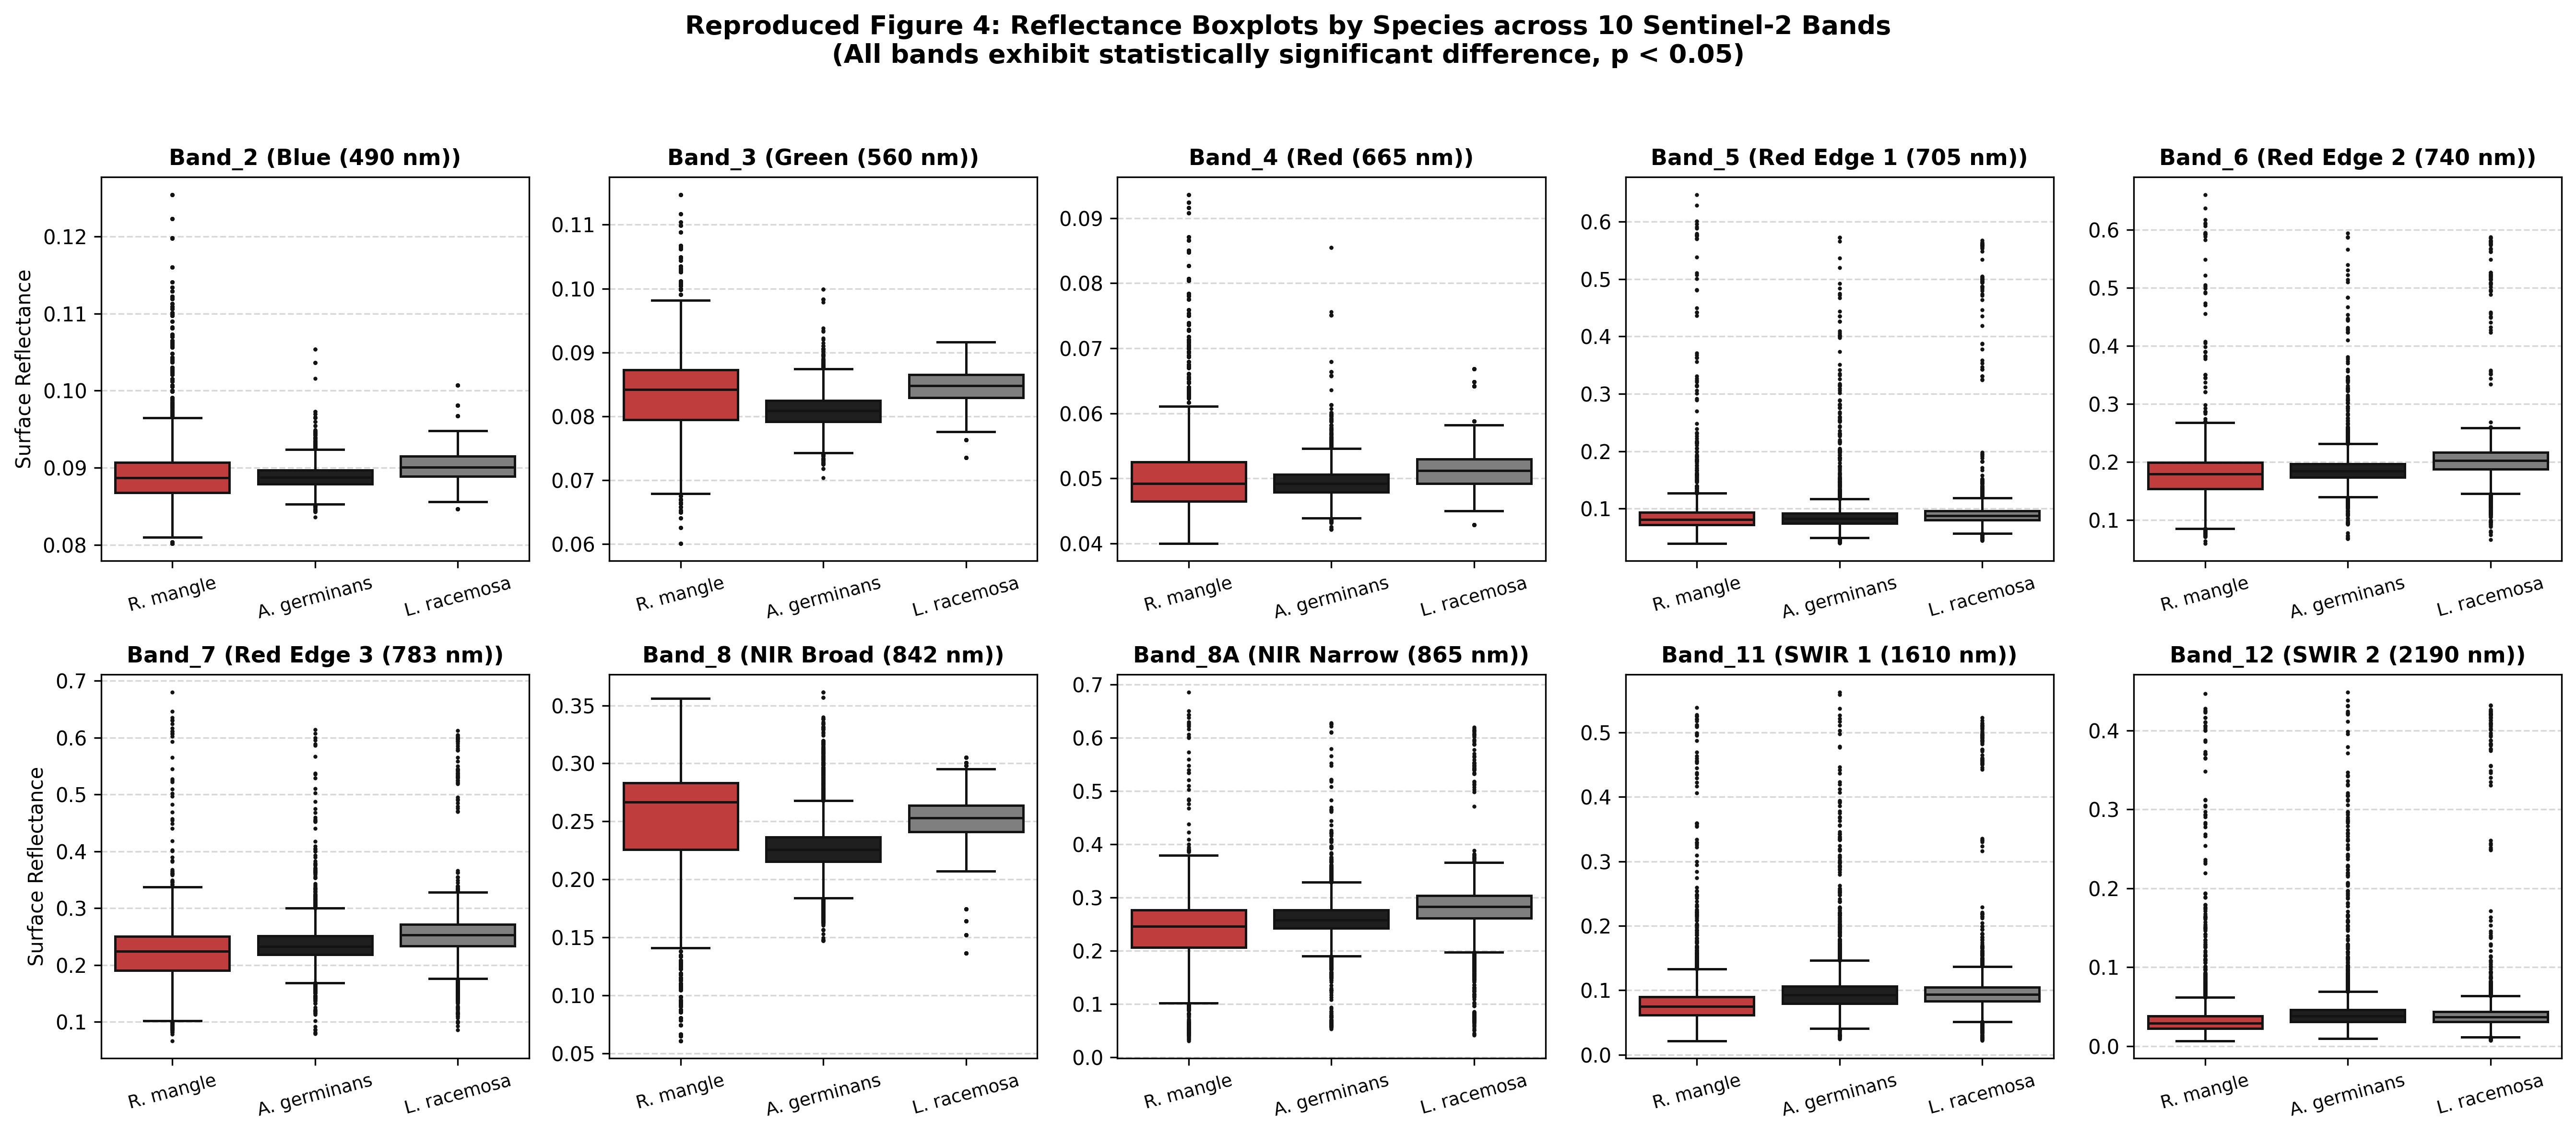
\includegraphics[width=0.96\textwidth]{figs/reproduced_figure4_boxplots.png}
\caption{Boxplots for each of the species (\emph{R.\ mangle}, \emph{A.\ germinans} and
\emph{L.\ racemosa}) by band, computed on the released monospecific dataset in this reproduction.
In all the comparisons there is a significant statistical difference between the species
($p<0.05$), qualitatively consistent with Fig.~4 of \citet{monterrubio2025} (see
Section~\ref{sec:threats} on the interpretation of significance at this sample size).}
\label{fig:boxplots}
\end{figure*}

\begin{figure}[!t]
\centering
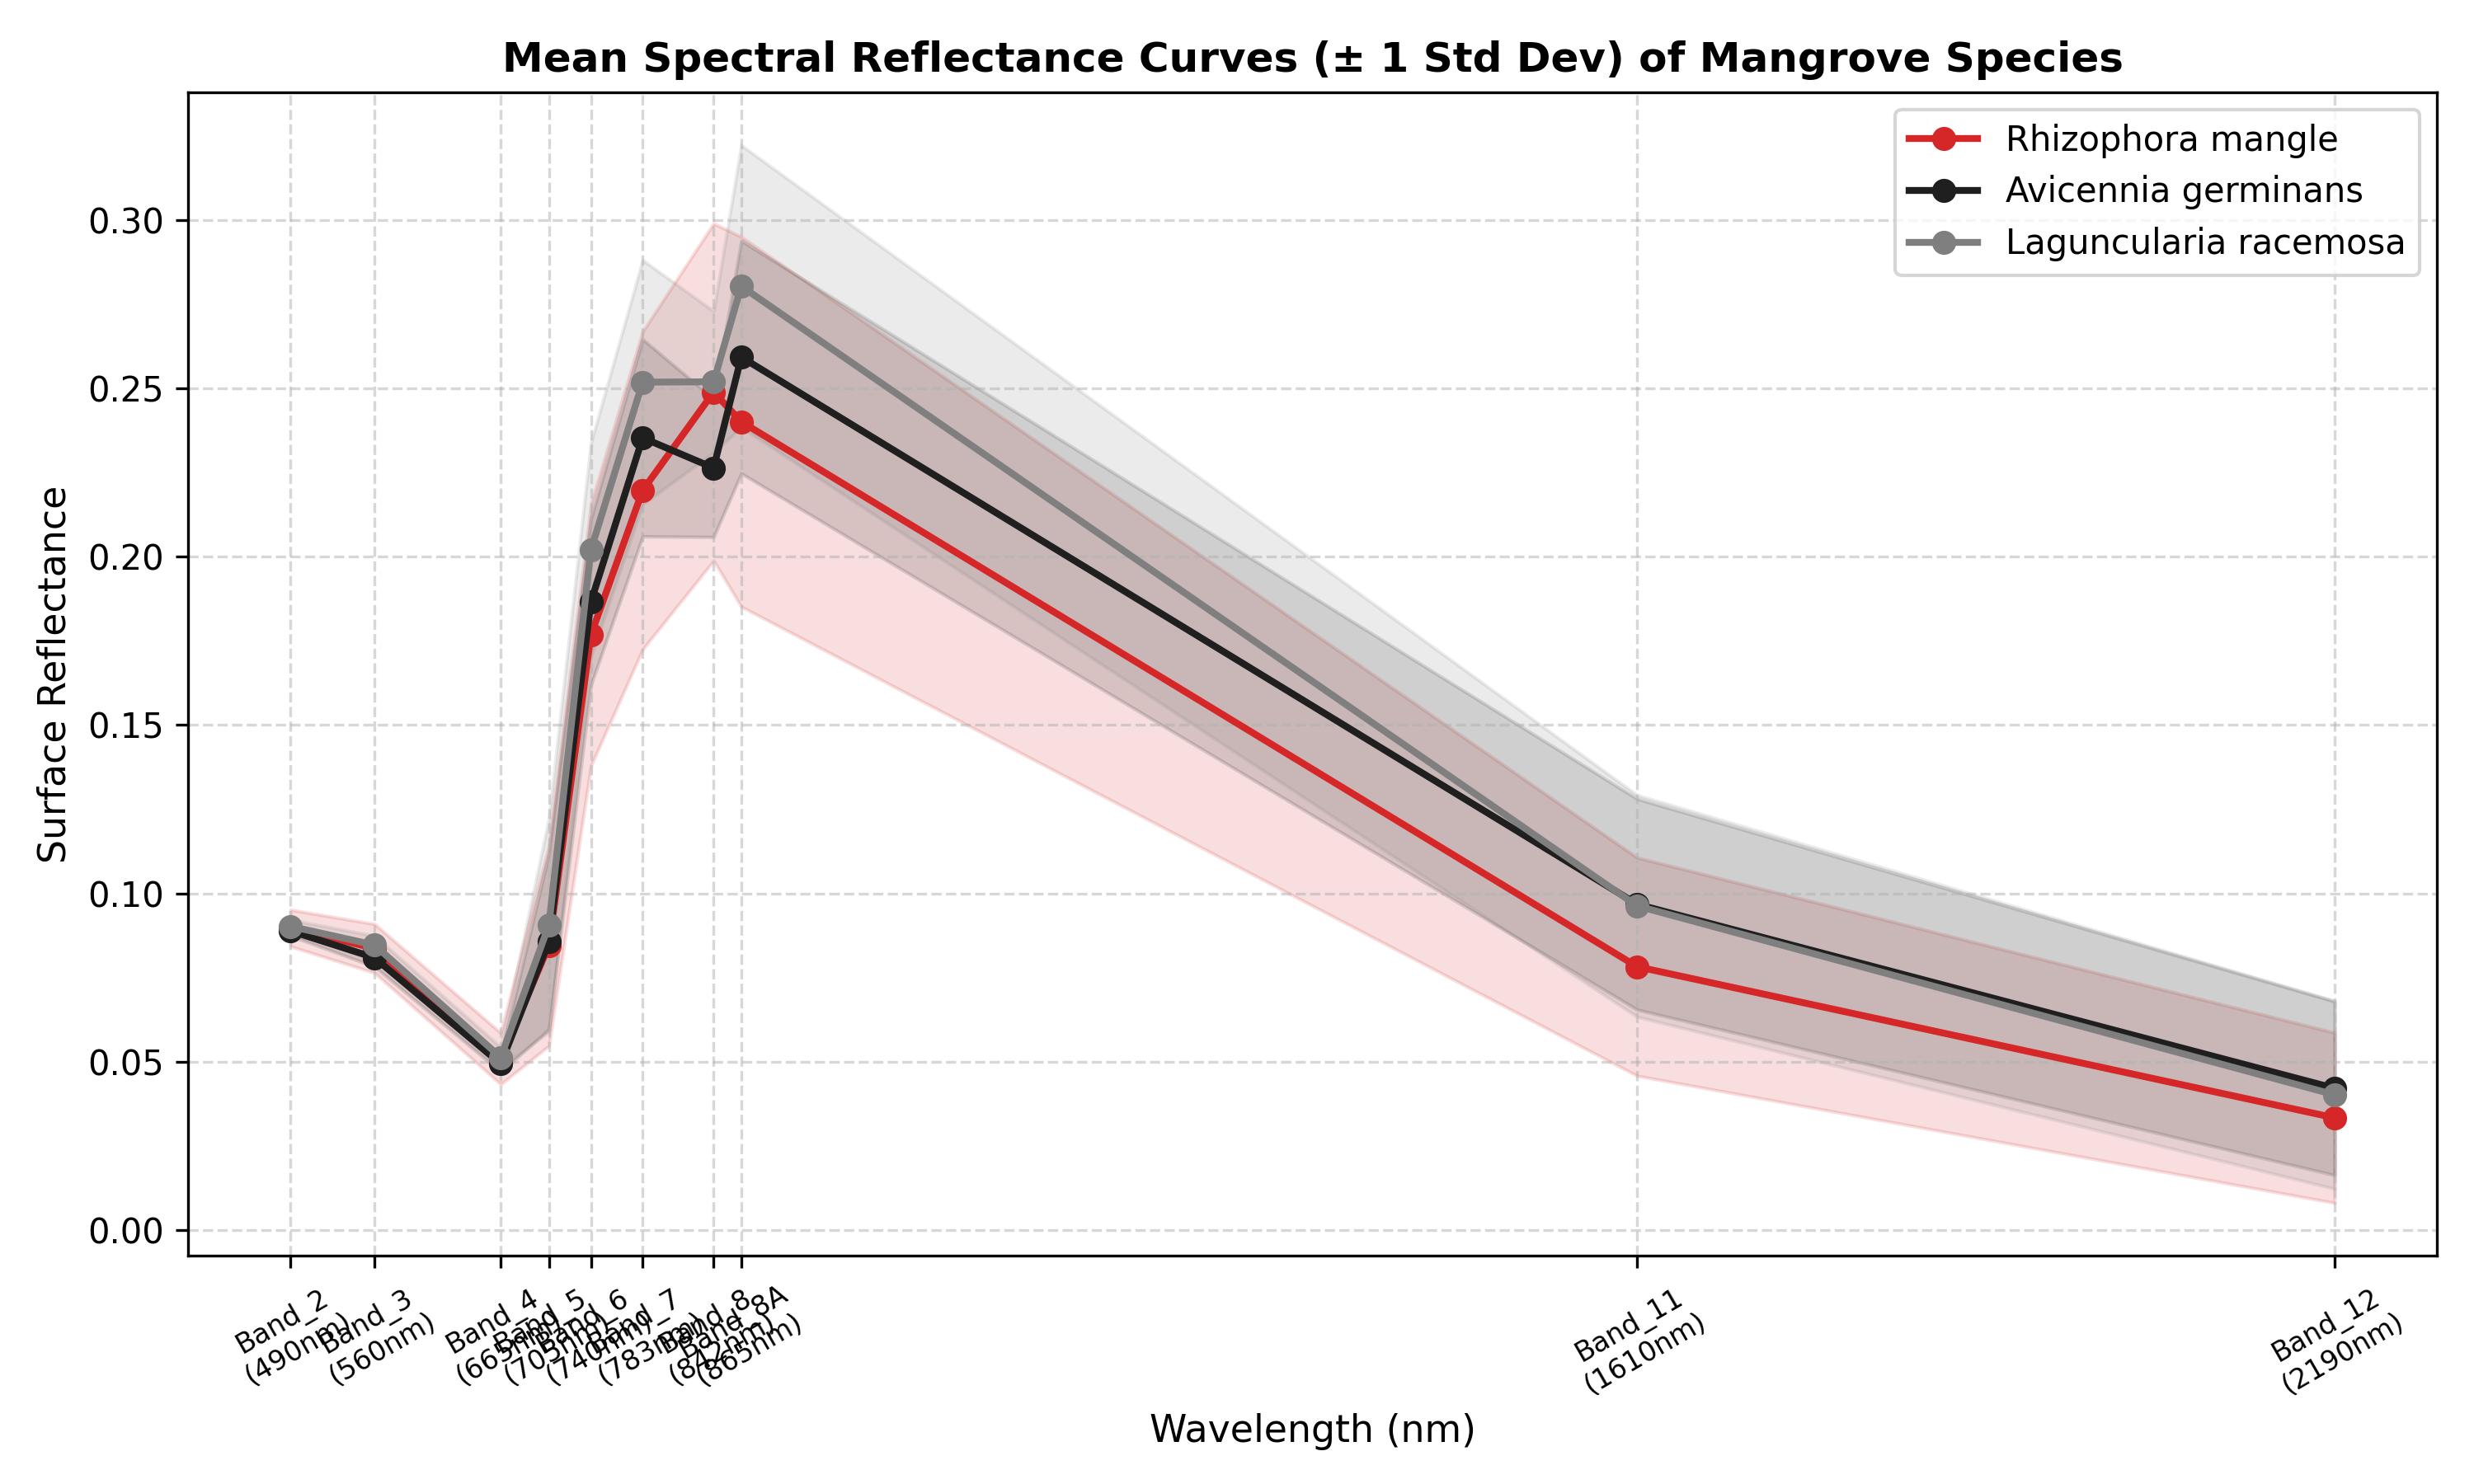
\includegraphics[width=\columnwidth]{figs/spectral_signatures.png}
\caption{Mean spectral reflectance curves ($\pm$ 1 standard deviation) of the three mangrove
species across the ten Sentinel-2 bands used by the models.}
\label{fig:signatures}
\end{figure}

\begin{figure*}[!t]
\centering
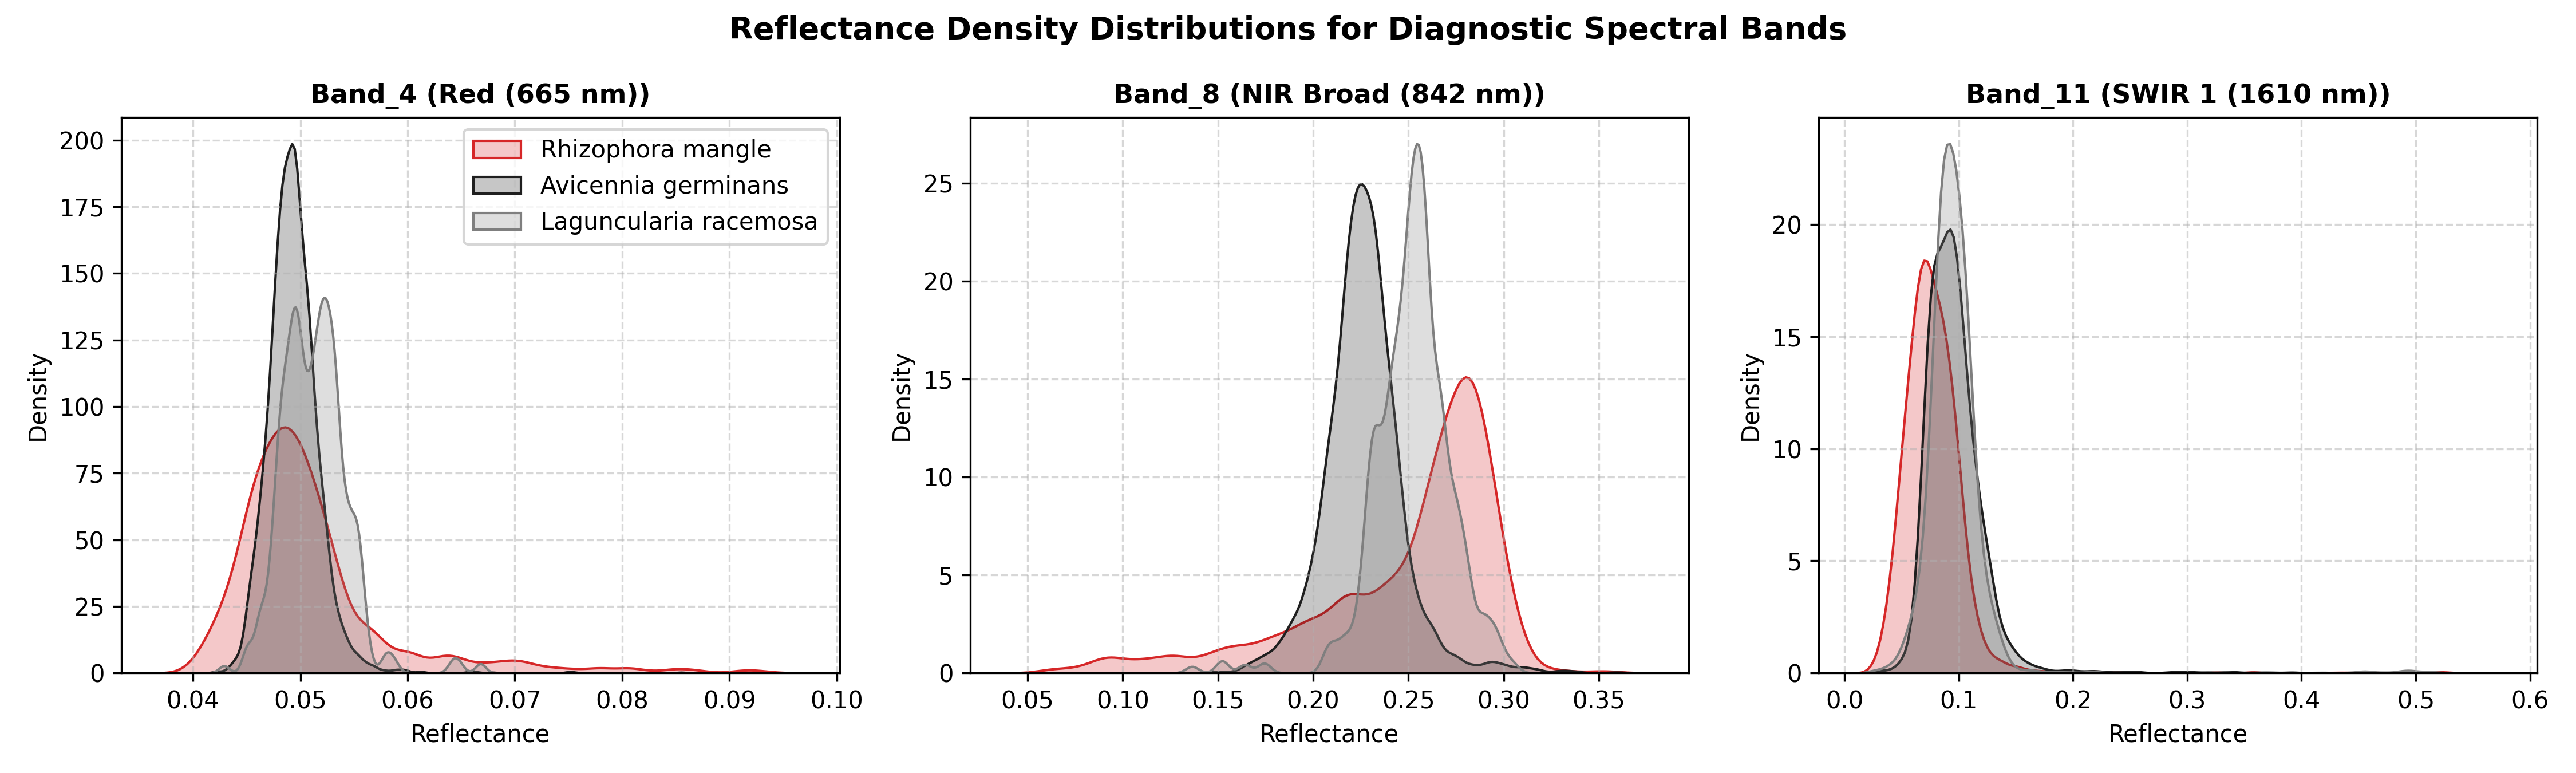
\includegraphics[width=0.96\textwidth]{figs/diagnostic_band_distributions.png}
\caption{Reflectance density distributions for the three most diagnostic spectral bands: red
(665\,nm), broad near-infrared (842\,nm) and first shortwave infrared (1610\,nm).}
\label{fig:densities}
\end{figure*}

\begin{figure}[!t]
\centering
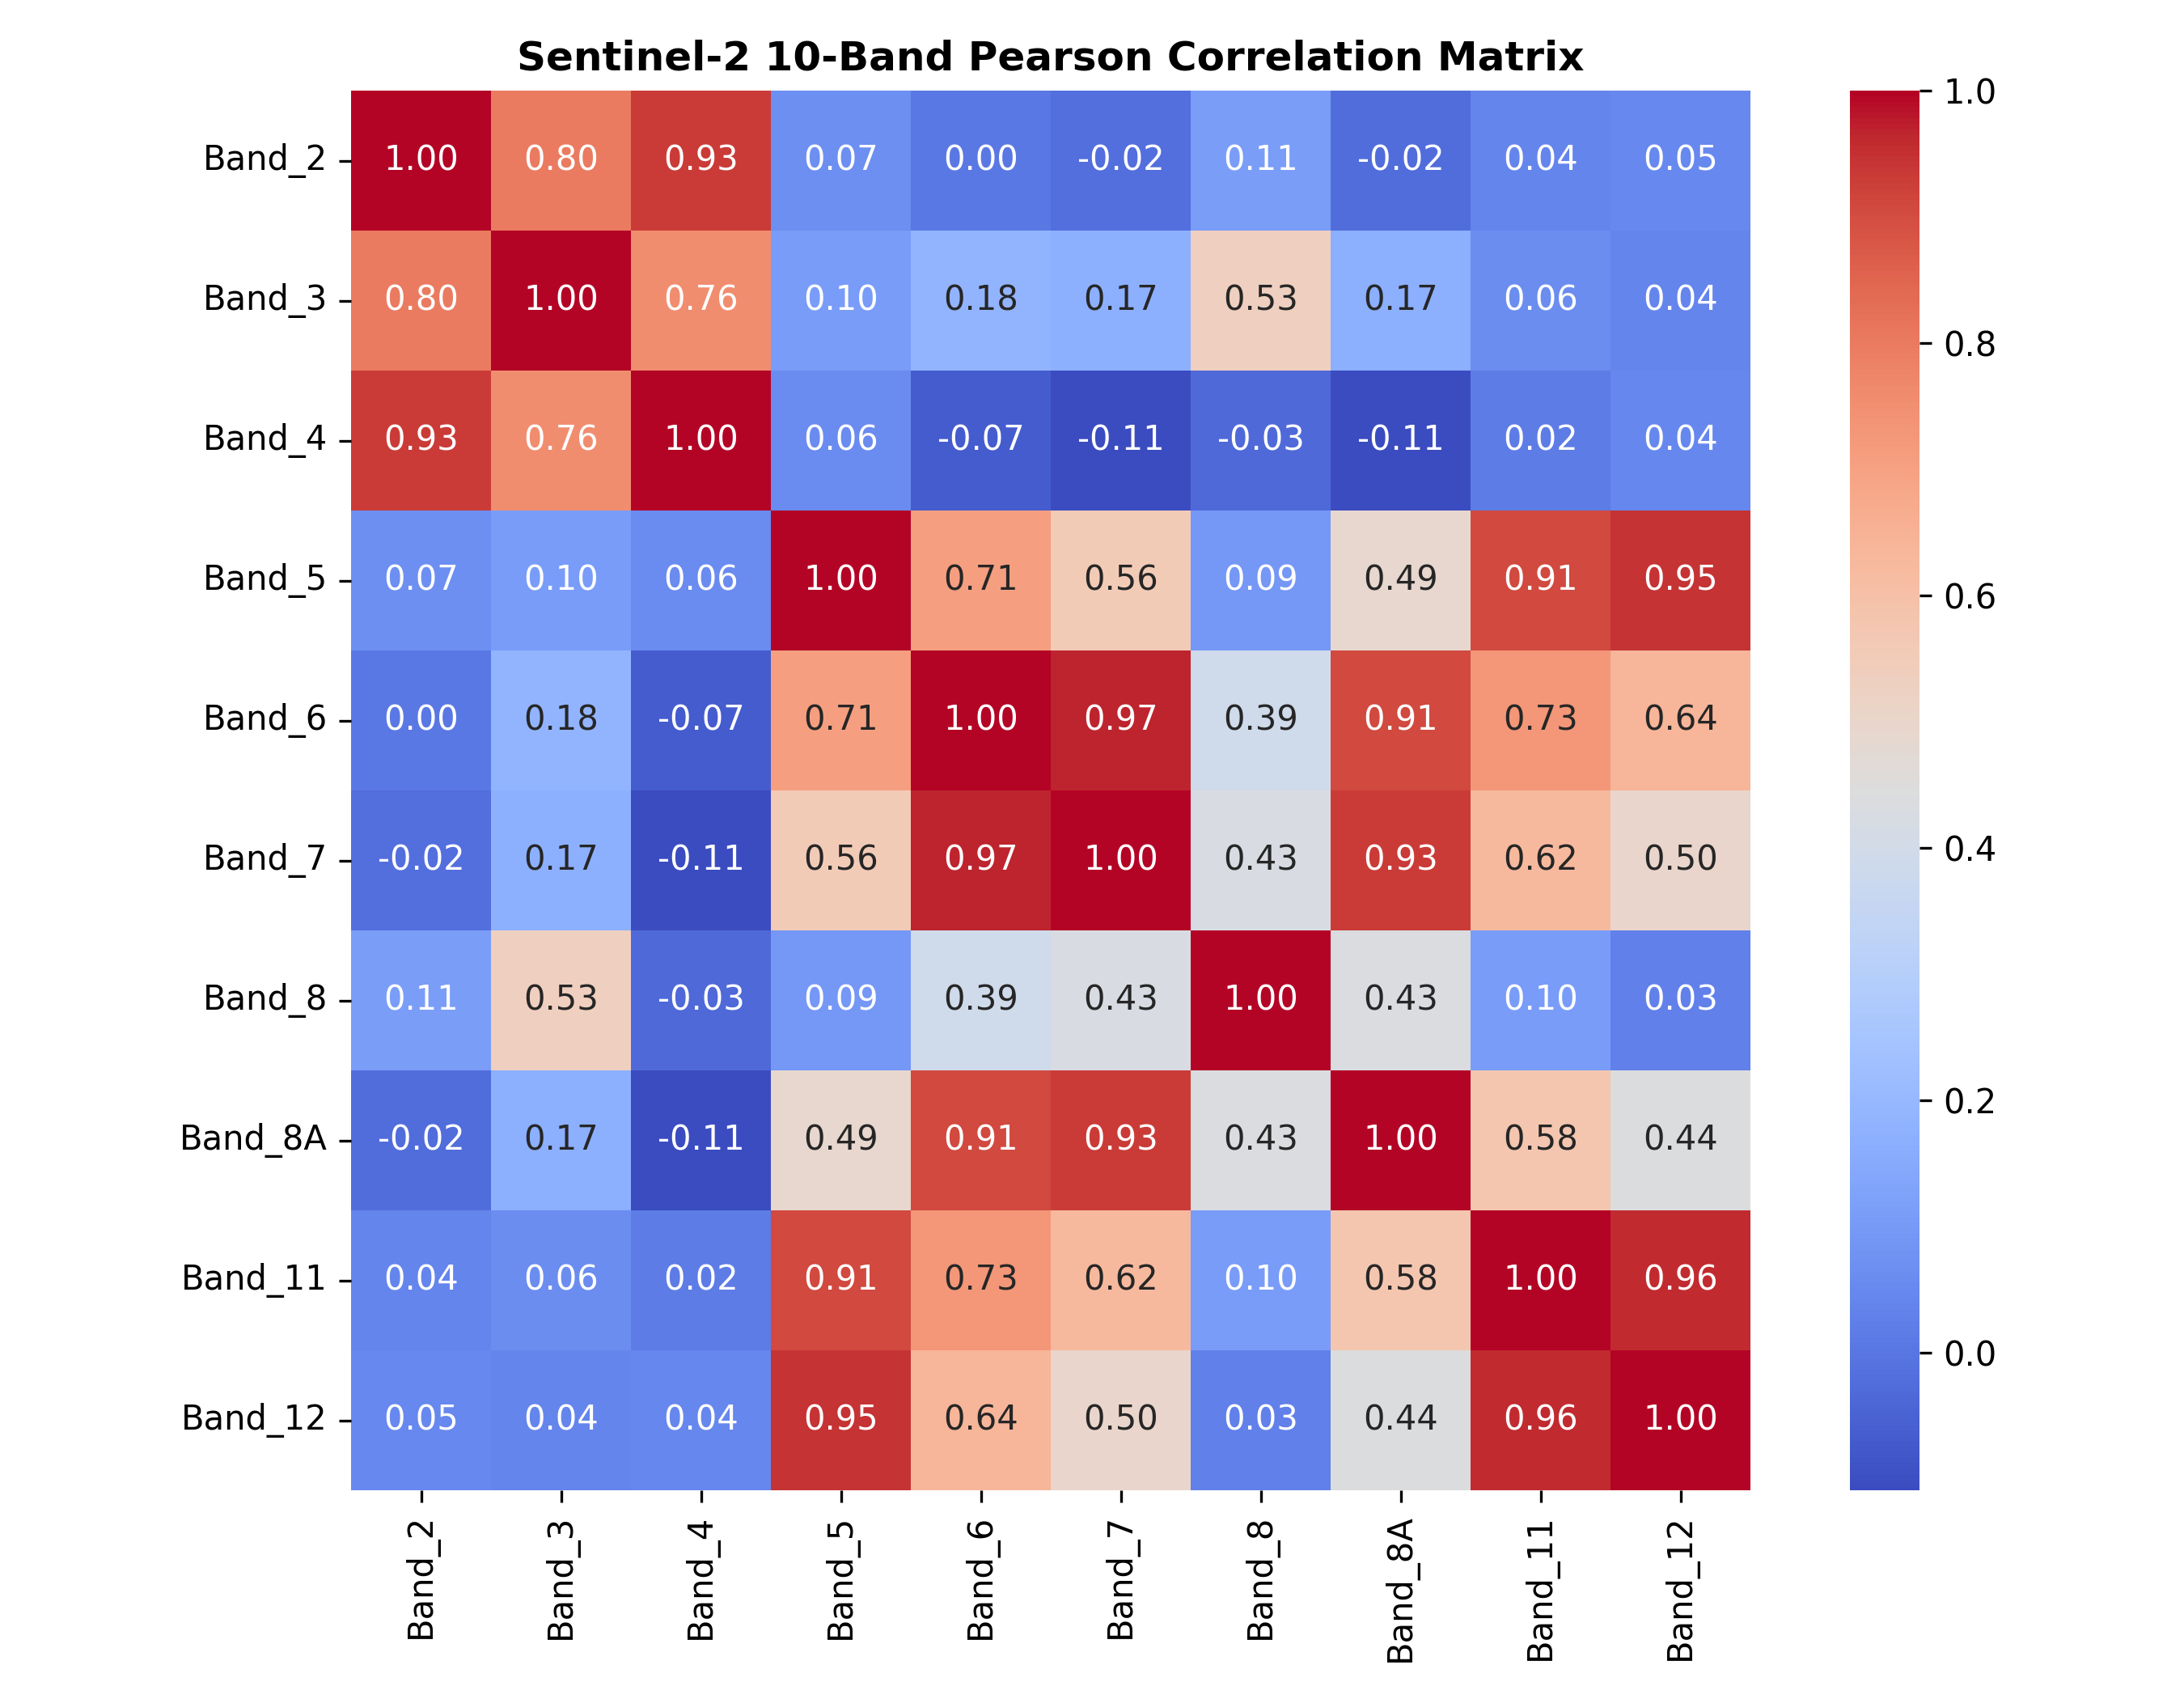
\includegraphics[width=\columnwidth]{figs/band_correlation_matrix.png}
\caption{Pearson correlation matrix of the ten Sentinel-2 bands over the monospecific mangrove
pixels, showing the visible and red-edge/shortwave infrared blocks.}
\label{fig:corr}
\end{figure}

\subsection{Multilayer perceptron models}
\label{sec:results-mlp}

Fig.~\ref{fig:paperacc} transcribes the accuracies reported by \citet{monterrubio2025} for both
tasks, which serve throughout as scientific reference benchmarks rather than as targets to be
matched. For the binary task all models exceed 0.990: the logistic model obtained the lowest
values, with a training accuracy of 0.9916 and a test accuracy of 0.9910, while one hidden layer
with 300 neurons reached 0.9995 and 0.9988, two hidden layers with 100 neurons 0.9994 and 0.9987,
three hidden layers with 50 neurons 0.9996 and 0.9987, four hidden layers with 150 and 300 neurons
0.9993 and 0.9986, and five hidden layers with 50 and 300 neurons 0.9995 and 0.9988; the
three-layer, 50-neuron model demonstrated the most optimal scores across all. For the four-class
task all models exceeded 0.90 except the logistic model, which obtained 0.7670 and 0.7684; the
three-layer, 500-neuron model reached 0.9863 and 0.9654 and the five-layer, 300-neuron model
0.9873 and 0.9684, while the five-layer, 50-neuron model obtained 0.9550 and 0.9454 and was
nevertheless identified by the authors as the most reliable of all models.
Table~\ref{tab:paper} lists these values in full.

Because the non-mangrove class is unavailable, neither the binary nor the four-class experiment of
the original study could be independently reproduced here. What could be executed is the identical
architectural grid, evaluated instead on the three-class monospecific subset of the released
pixels. Table~\ref{tab:ours} reports the outcome for the ten configurations that the original
article discusses numerically. Test accuracy under the pixel-level holdout described in
Section~\ref{sec:methods-mlp} rises from 0.6964 for the logistic baseline to 0.8740 for a single hidden layer of 500
neurons, and reaches a maximum of 0.9498 for four hidden layers of 300 neurons among the
configurations evaluated. This indicates that, under this experimental setup, the three mangrove
species --- which share canopy architecture, phenology and inundation regime --- are separable at
better than 94\,\% from ten bands of reflectance alone, without any vegetation index, which is
consistent with the central spectral premise of the original study.

Figs.~\ref{fig:scaling3} and \ref{fig:scaling} describe how accuracy depends on depth and width
across the full 41-model grid. Mean test accuracy across widths increases from 69.64\,\% for the
logistic baseline to 83.84\,\% at one hidden layer, 87.82\,\% at two, 89.28\,\% at three and
89.96\,\% at four, and then falls slightly to 88.89\,\% at five. Depth beyond four layers
therefore yields no further gain in tabular accuracy. Width behaves differently: mean test accuracy
climbs steeply from 79.81\,\% at 5 neurons to 91.80\,\% at 100, then flattens at 93.12\,\% for
150, 94.16\,\% for 300 and 94.38\,\% for 500, so the last threefold increase in width buys roughly
one percentage point while parameter count and training time grow by an order of magnitude. Both
patterns are consistent with the low effective dimensionality of the correlated band set in
Fig.~\ref{fig:corr}.

\textbf{NOT A DIRECT PERFORMANCE COMPARISON.} Fig.~\ref{fig:compare} places the reproduced
three-species accuracies alongside the four-class accuracies reported by the authors, with the
difference in percentage points annotated above each pair, purely for audit transparency. The two
sets of values are computed on different class spaces (three mangrove species here versus three
species plus a non-mangrove background class in the original study), with different class priors
and different chance baselines (33.3\,\% against 25\,\%), and are not directly comparable as
measures of model quality in either direction. The reproduced values are lower for every
architecture, by between 1.04 and 7.20 percentage points, with a mean offset of $-3.09$ percentage
points (Table~\ref{tab:diff}). A plausible, though not separately tested, explanation is that the
original task contained a non-mangrove background class comprising a quarter of all samples, and
that water, bare dunes and urban surfaces are typically far more separable from green canopy in
reflectance space than three co-occurring mangrove species are from one another; a four-class
problem in which one class is comparatively easy to classify would raise overall accuracy
mechanically relative to a three-class problem restricted to mangrove species. The largest offset
occurs for the logistic baseline ($-7.20$ pp), consistent with this explanation, but the offset
itself should be read as a consequence of the differing class space and evaluation design, not as
evidence that either implementation is more or less accurate as a classifier.

\begin{figure*}[!t]
\centering
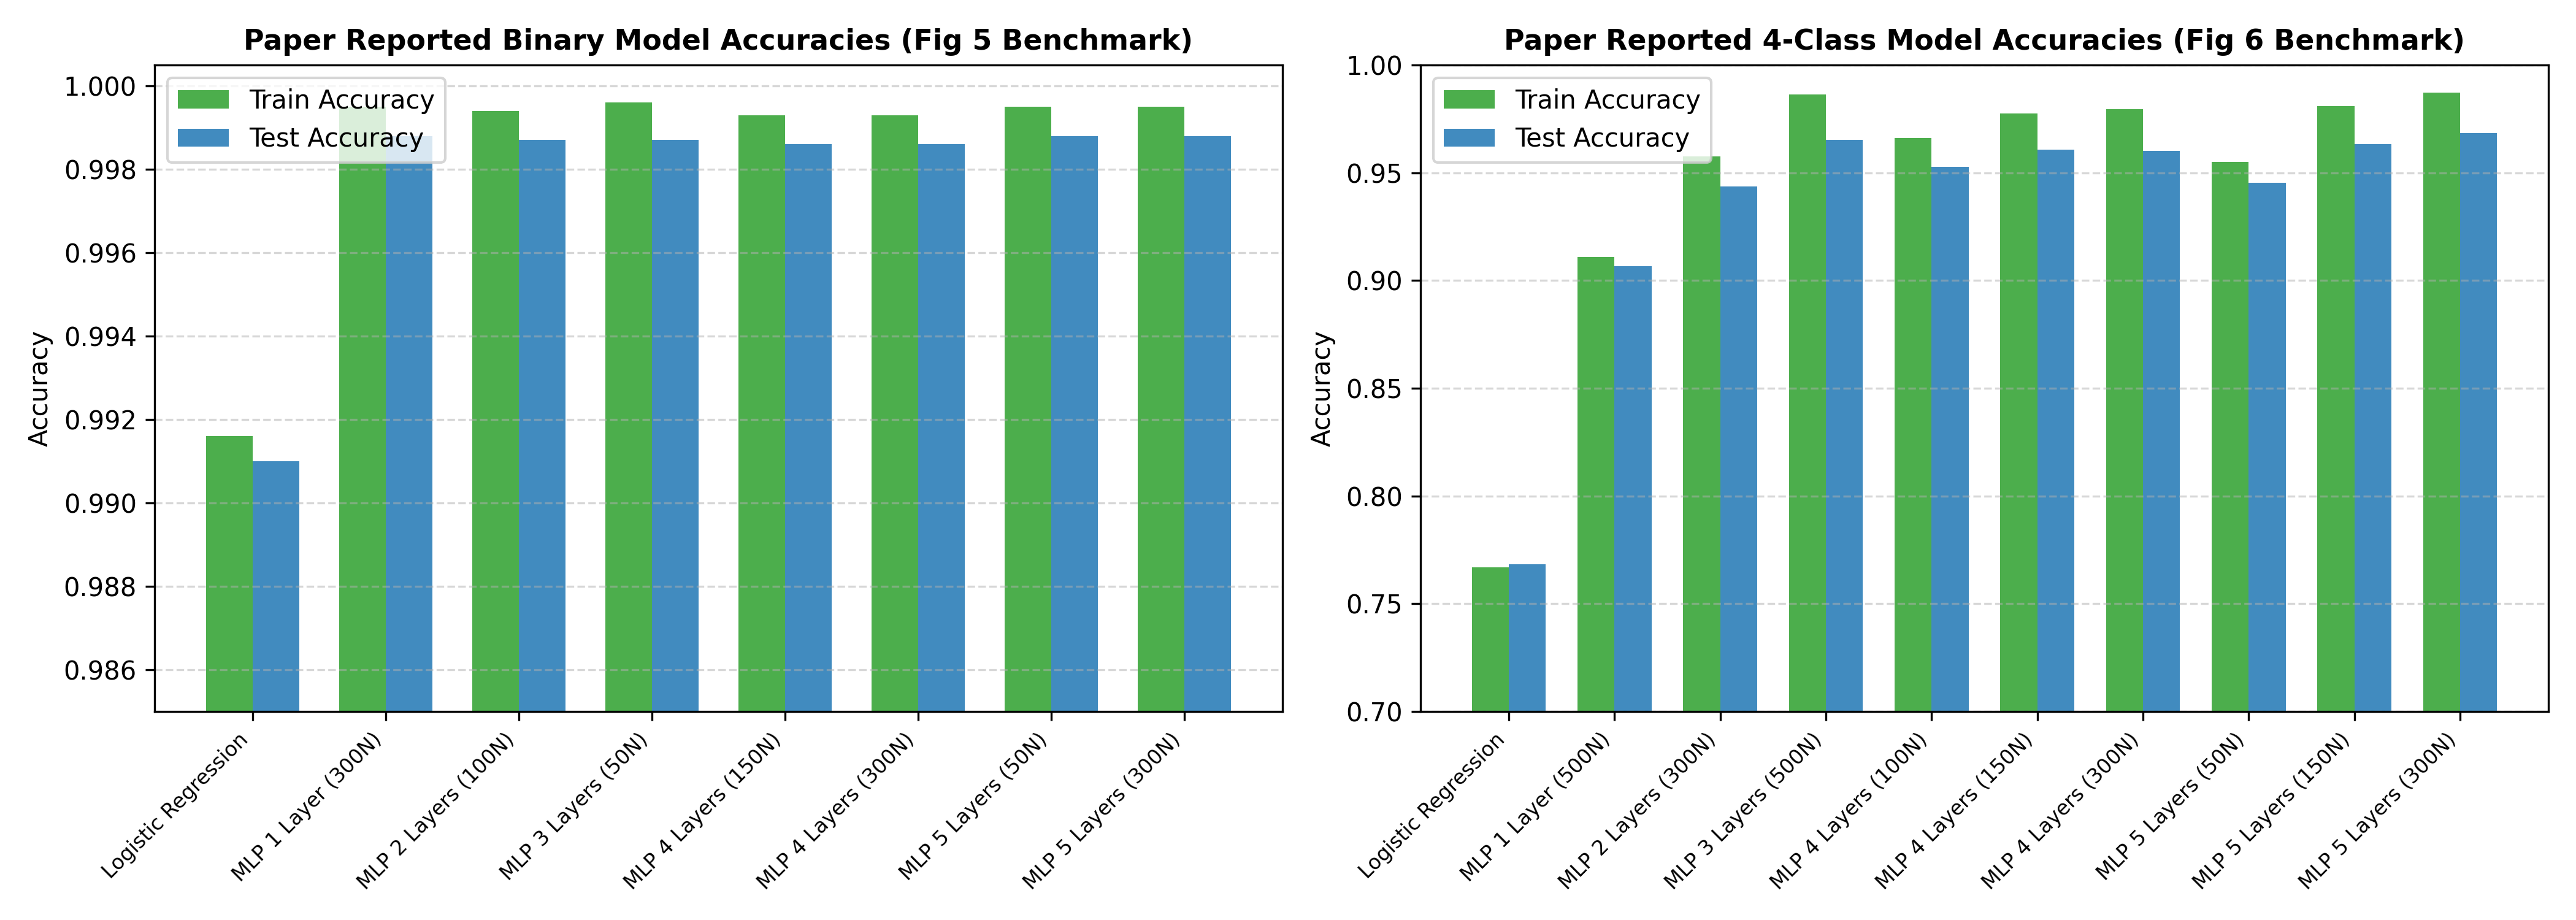
\includegraphics[width=0.96\textwidth]{figs/paper_reported_accuracies_summary.png}
\caption{Accuracies reported by \citet{monterrubio2025} for the binary 60{,}000-pixel models
(left, their Fig.~5) and the four-class 40{,}000-pixel models (right, their Fig.~6), transcribed
here as reference benchmarks.}
\label{fig:paperacc}
\end{figure*}

\begin{figure*}[!t]
\centering
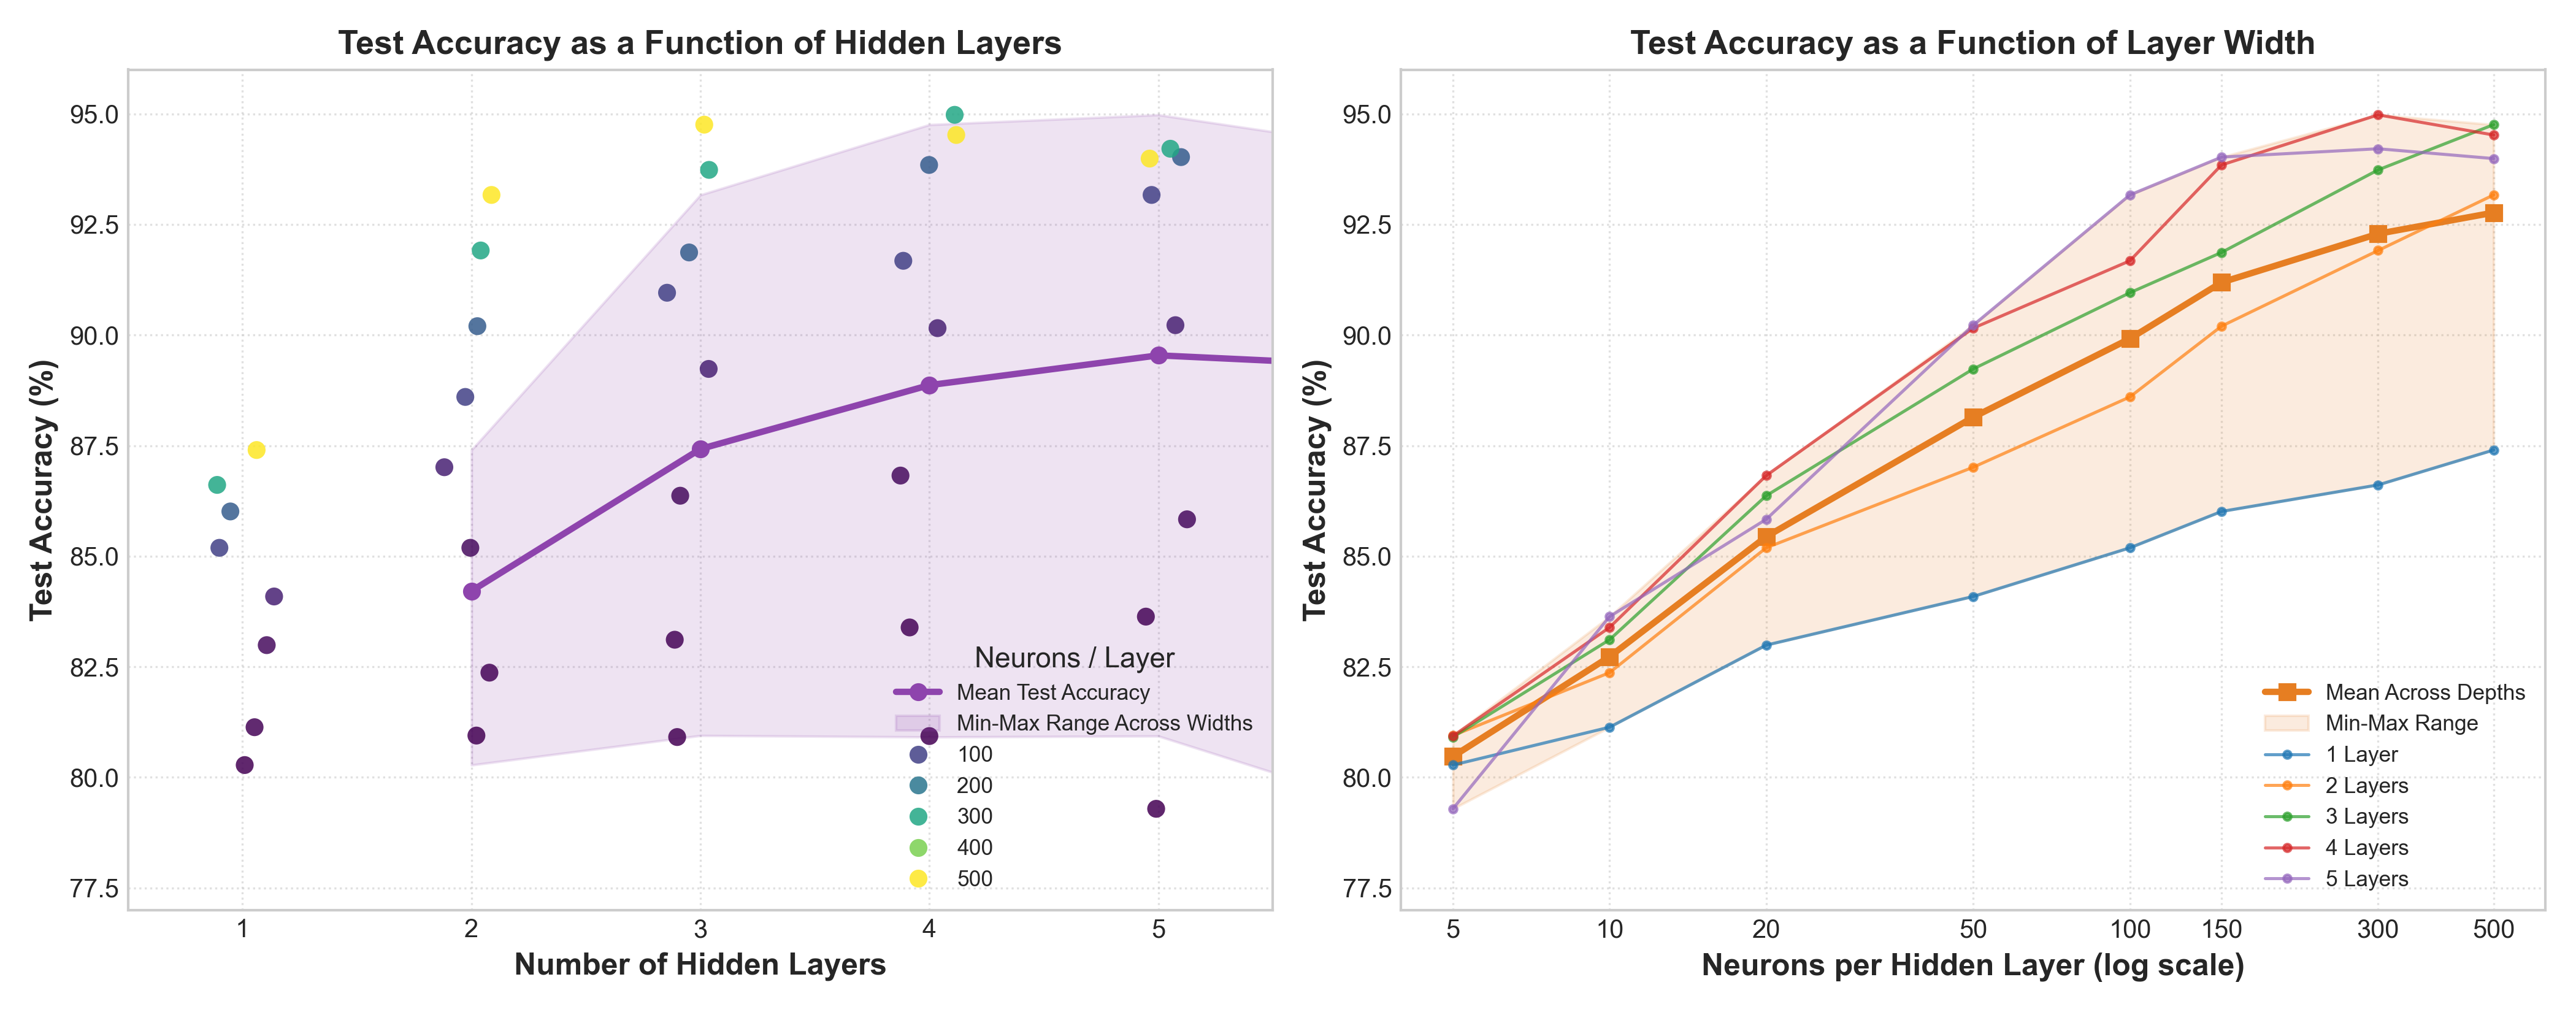
\includegraphics[width=0.96\textwidth]{figs/accuracy_by_layer_and_neurons.png}
\caption{Test accuracy of the reproduced three-species models as a function of hidden-layer depth
(left) and of layer width (right) across the complete 41-configuration grid.}
\label{fig:scaling}
\end{figure*}

\begin{figure}[!t]
\centering
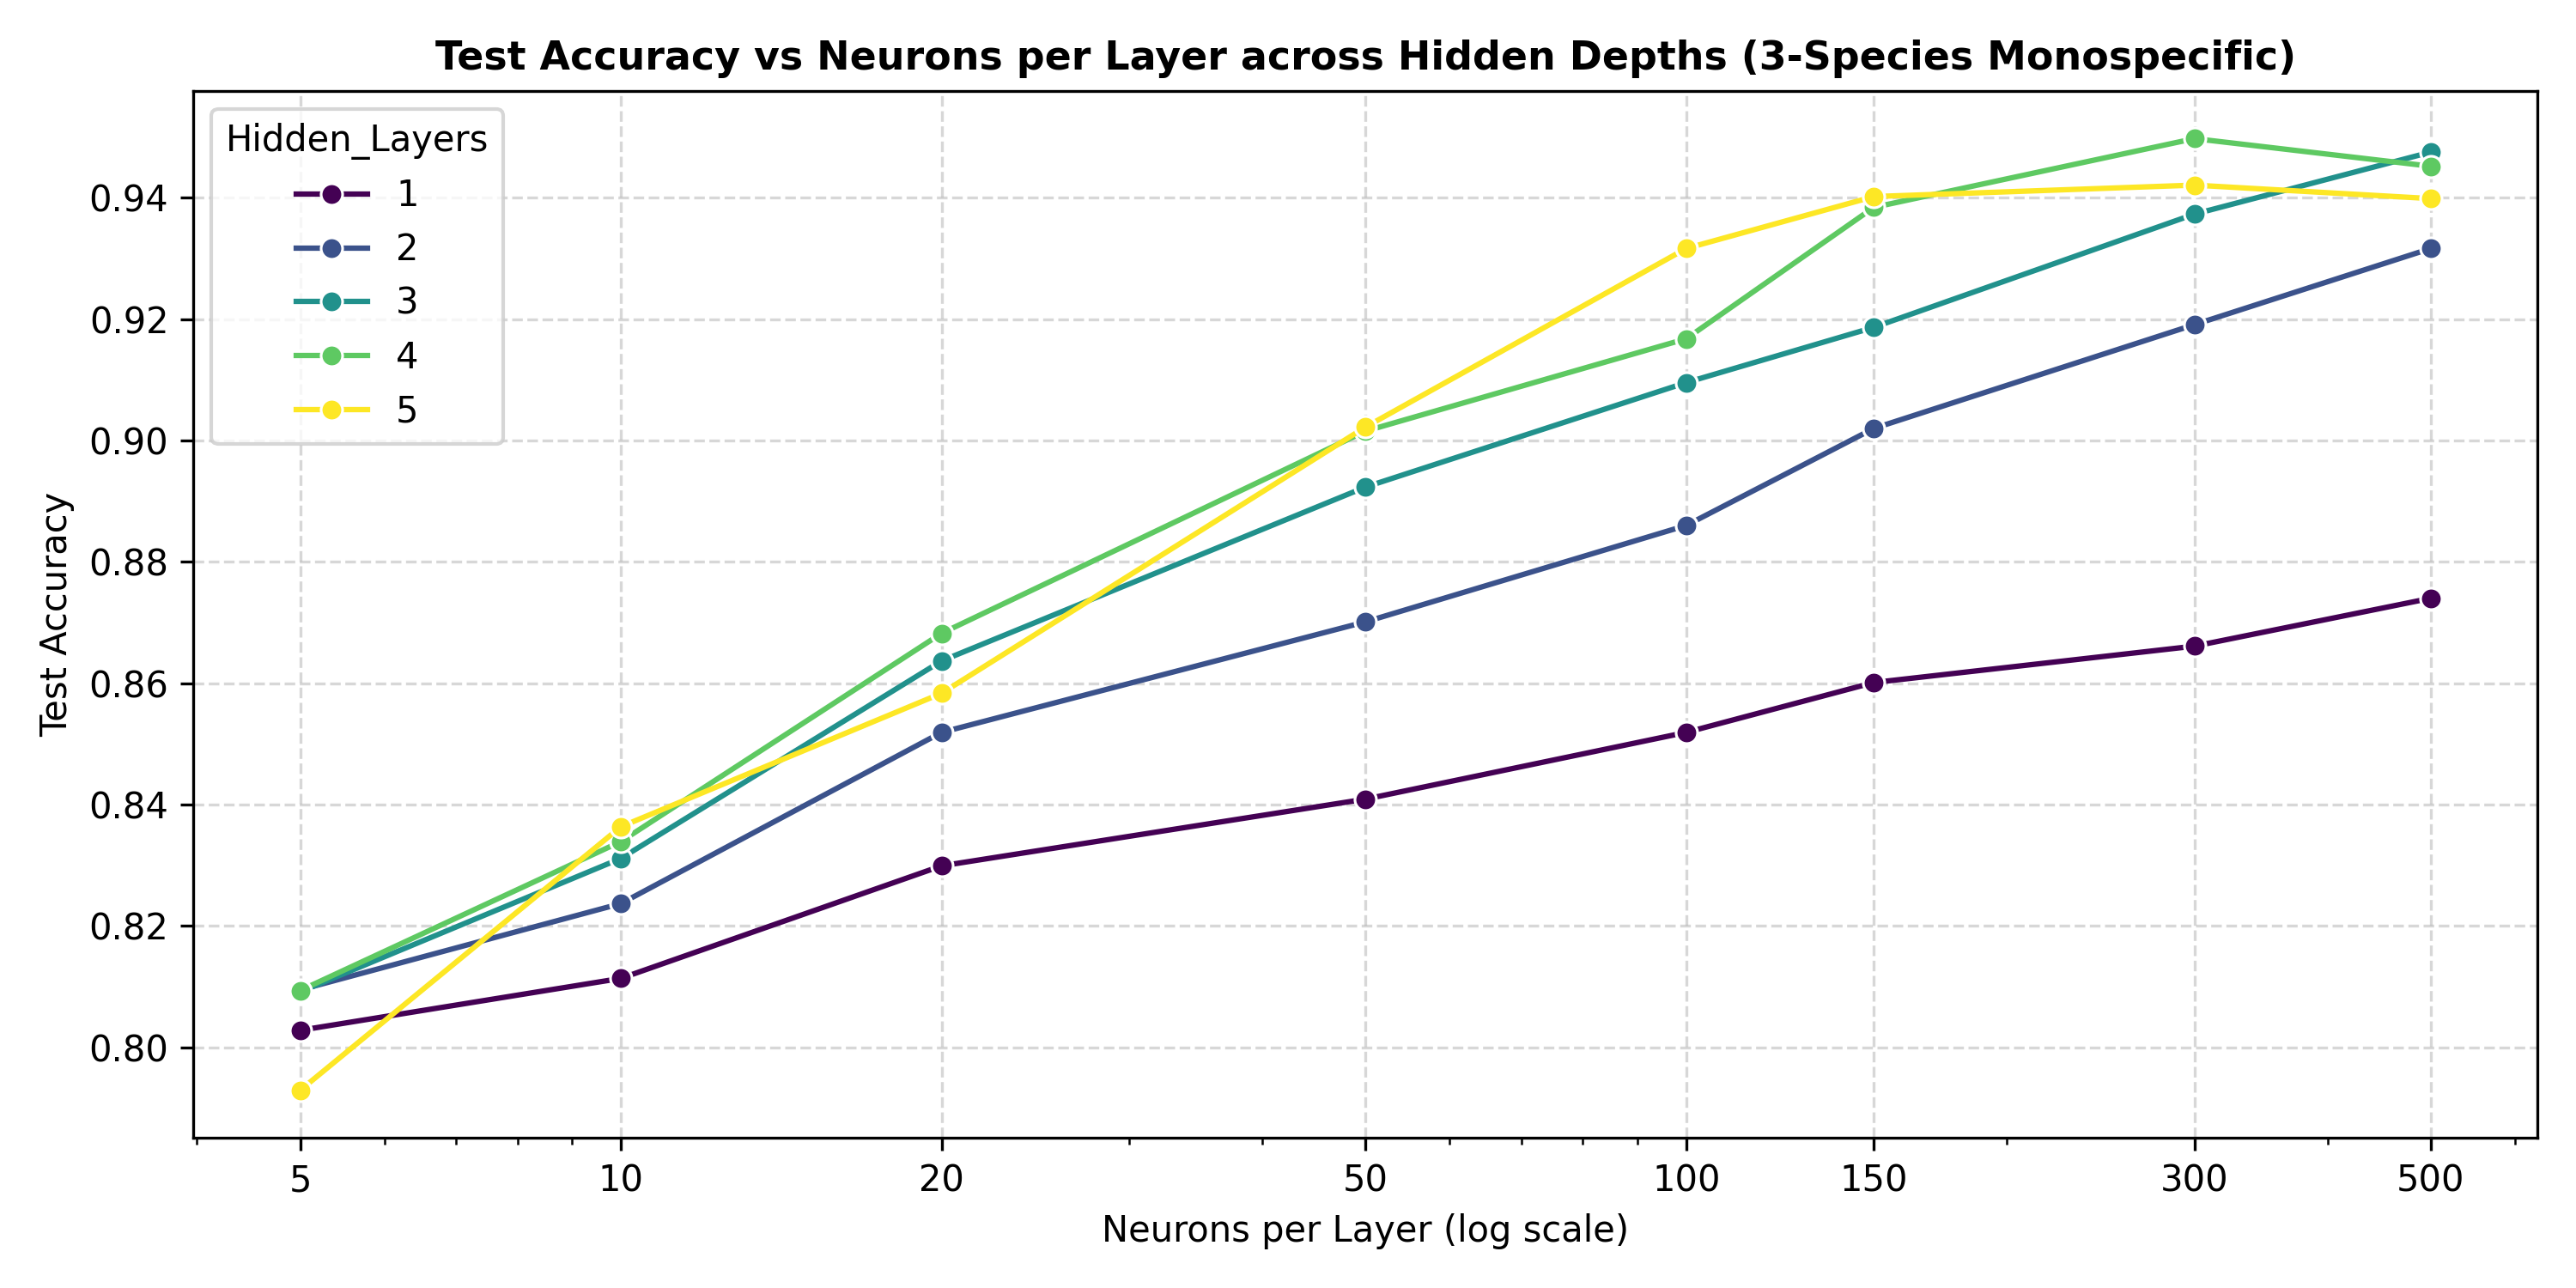
\includegraphics[width=\columnwidth]{figs/depth_width_scaling_3species.png}
\caption{Test accuracy against neurons per layer for each hidden-layer depth on the three-species
monospecific dataset.}
\label{fig:scaling3}
\end{figure}

\begin{figure*}[!t]
\centering
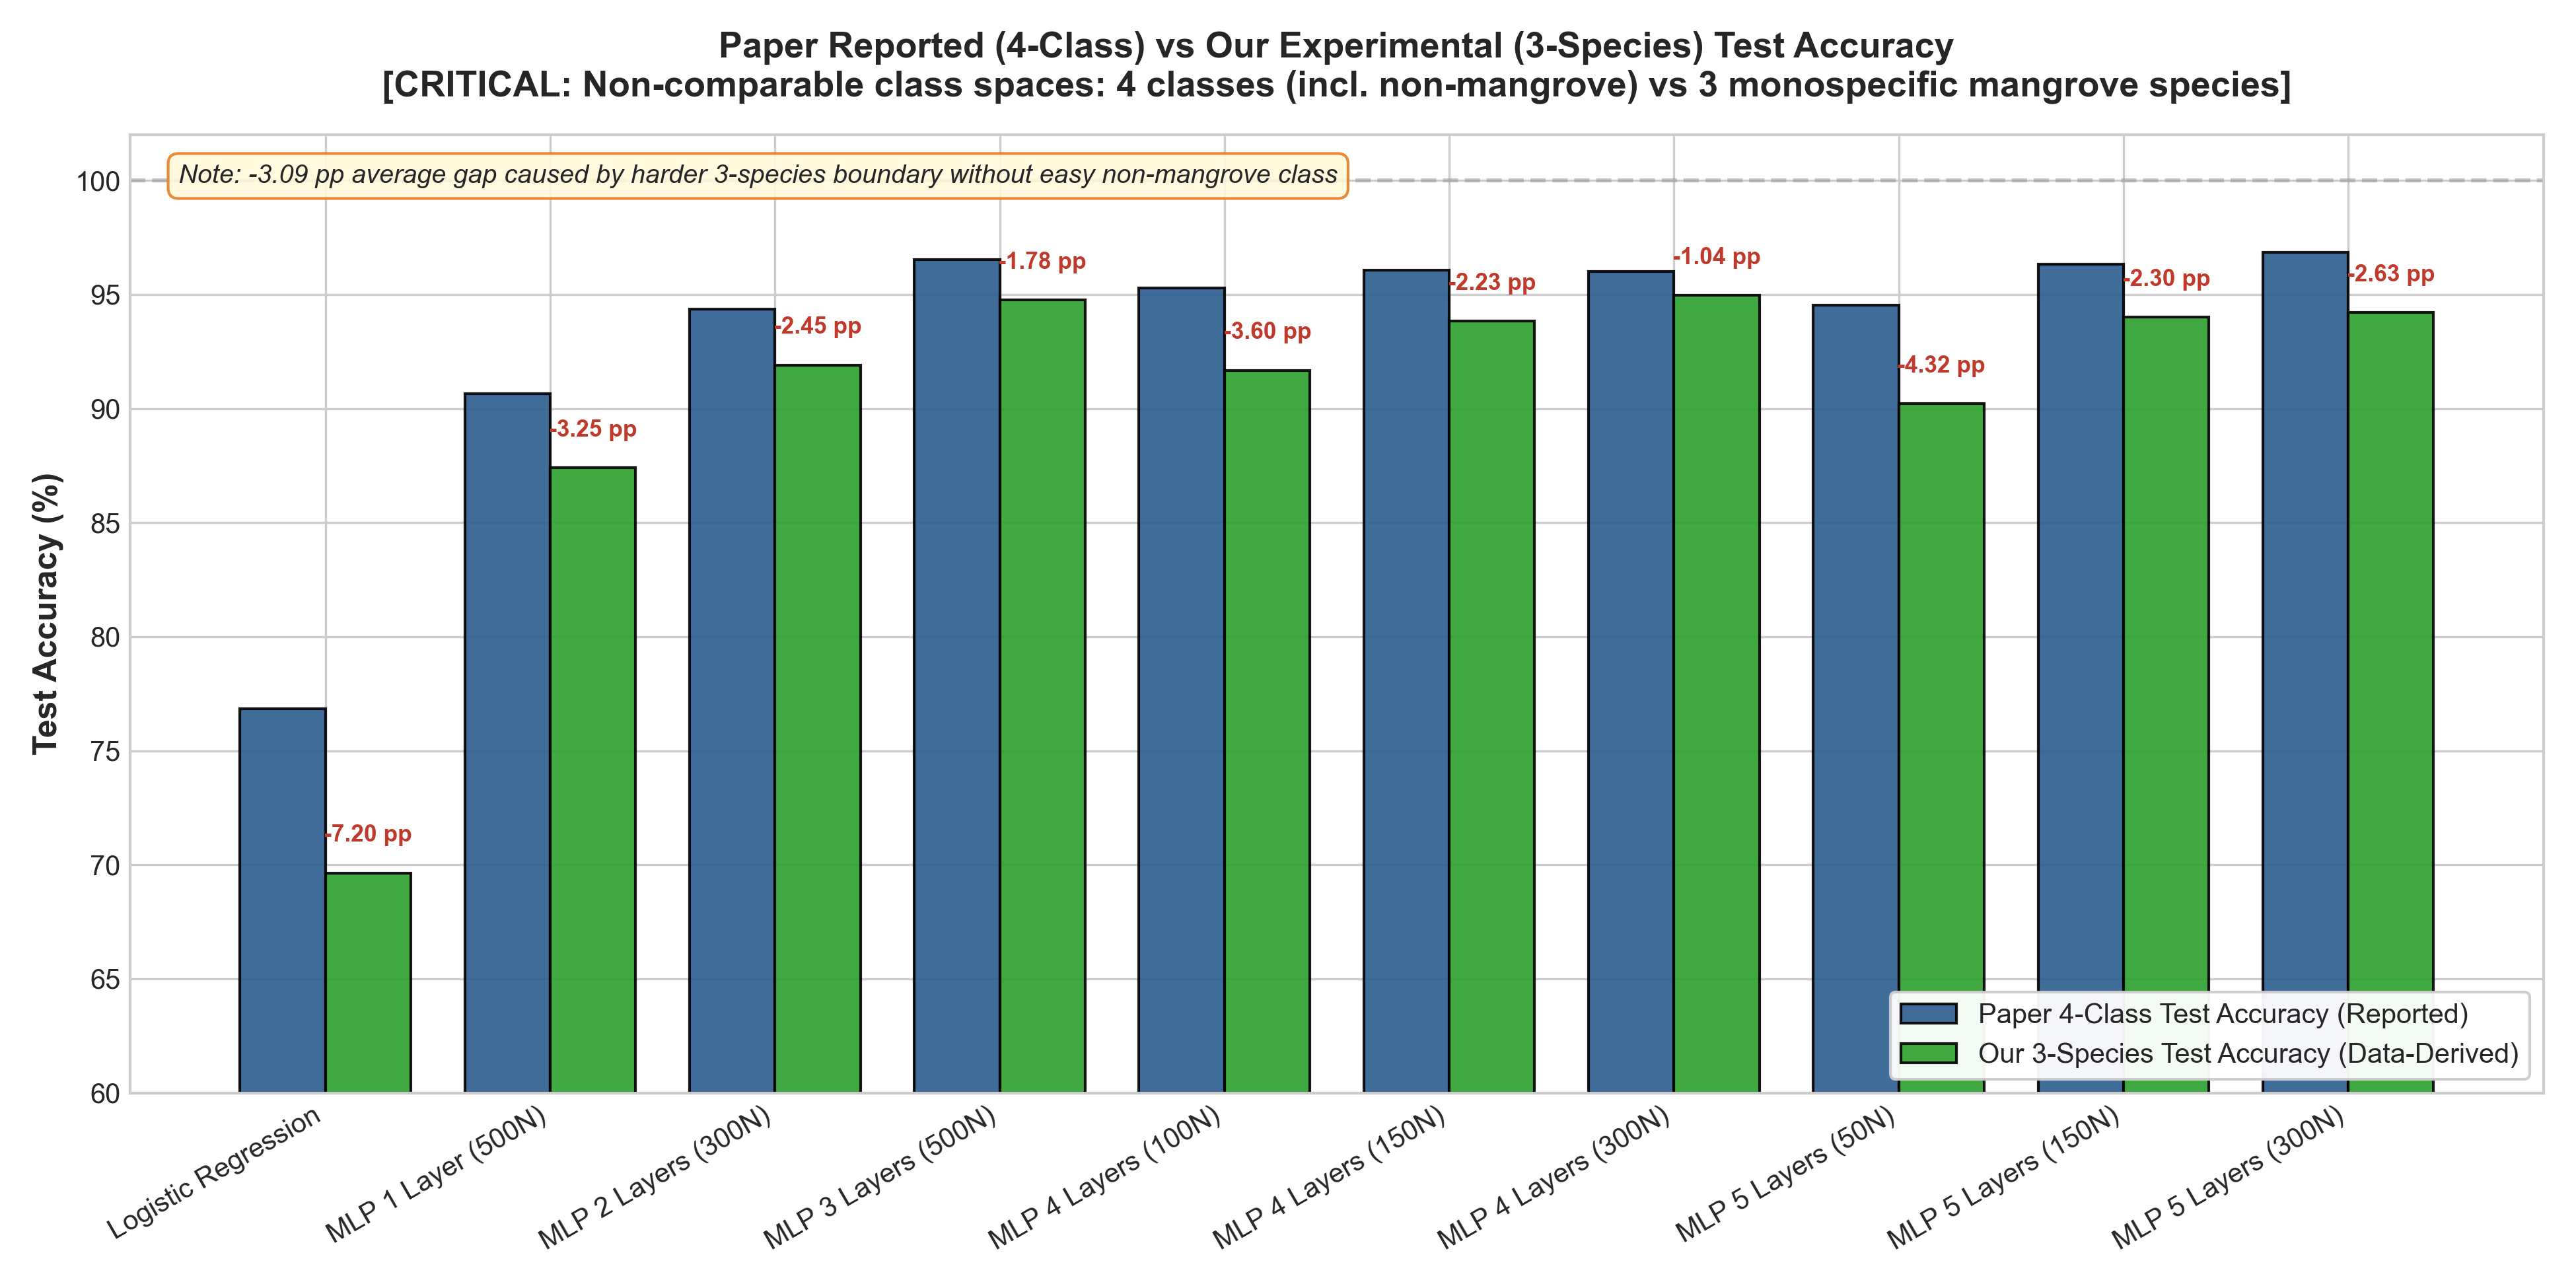
\includegraphics[width=0.96\textwidth]{figs/paper_vs_our_accuracy_comparison.png}
\caption{\textbf{Not a direct performance comparison.} Four-class test accuracies reported by
\citet{monterrubio2025} against the three-species test accuracies obtained in this reproduction,
with the percentage-point difference annotated. The two class spaces differ (three mangrove species
here versus three species plus a non-mangrove background class in the original study), so the
values are shown for audit transparency only and must not be read as a measure of relative model
quality.}
\label{fig:compare}
\end{figure*}

\begin{table}[!t]
\centering
\caption{Accuracies reported by \citet{monterrubio2025} for the binary (60{,}000 pixels) and
four-class (40{,}000 pixels) tasks.}
\label{tab:paper}
\footnotesize
\setlength{\tabcolsep}{3.4pt}
\begin{tabular}{l c c c c}
\toprule
\multirow{2}{*}{\textbf{Architecture}} & \multicolumn{2}{c}{\textbf{Binary}} & \multicolumn{2}{c}{\textbf{Four-class}} \\
\cmidrule(lr){2-3}\cmidrule(lr){4-5}
 & Train & Test & Train & Test \\
\midrule
Logistic regression & 0.9916 & 0.9910 & 0.7670 & 0.7684 \\
1 layer, 300 neurons & 0.9995 & 0.9988 & --- & --- \\
1 layer, 500 neurons & --- & --- & 0.9110 & 0.9065 \\
2 layers, 100 neurons & 0.9994 & 0.9987 & --- & --- \\
2 layers, 300 neurons & --- & --- & 0.9575 & 0.9436 \\
3 layers, 50 neurons & 0.9996 & 0.9987 & --- & --- \\
3 layers, 500 neurons & --- & --- & 0.9863 & 0.9654 \\
4 layers, 100 neurons & --- & --- & 0.9662 & 0.9528 \\
4 layers, 150 neurons & 0.9993 & 0.9986 & 0.9775 & 0.9607 \\
4 layers, 300 neurons & 0.9993 & 0.9986 & 0.9795 & 0.9602 \\
5 layers, 50 neurons & 0.9995 & 0.9988 & 0.9550 & 0.9454 \\
5 layers, 150 neurons & --- & --- & 0.9810 & 0.9632 \\
5 layers, 300 neurons & 0.9995 & 0.9988 & 0.9873 & 0.9684 \\
\bottomrule
\end{tabular}
\end{table}

\begin{table}[!t]
\centering
\caption{Reproduced results on the class-balanced three-species monospecific dataset
(30{,}000 pixels; 21{,}000 train / 9{,}000 test), under the stratified pixel-level holdout described
in Section~\ref{sec:methods-mlp}. Parameter counts as recorded in the reproduction results table
(\texttt{three\_class\_mangrove\_results.csv}); see the parameter-count footnote in Section~\ref{sec:gap} on a minor discrepancy
with the rounded figure-annotation value for MLP~5L--50N.}
\label{tab:ours}
\footnotesize
\setlength{\tabcolsep}{3.2pt}
\begin{tabular}{l c c c c c}
\toprule
\textbf{Model} & \textbf{L} & \textbf{N} & \textbf{Params} & \textbf{Train} & \textbf{Test} \\
\midrule
Logistic baseline & 0 & --- & 33 & 0.6989 & 0.6964 \\
MLP 1L--500N & 1 & 500 & 7{,}003 & 0.8807 & 0.8740 \\
MLP 2L--300N & 2 & 300 & 94{,}203 & 0.9611 & 0.9191 \\
MLP 3L--500N & 3 & 500 & 508{,}003 & 0.9946 & 0.9476 \\
MLP 4L--100N & 4 & 100 & 31{,}503 & 0.9593 & 0.9168 \\
MLP 4L--150N & 4 & 150 & 70{,}053 & 0.9824 & 0.9384 \\
MLP 4L--300N & 4 & 300 & 274{,}803 & 0.9948 & \textbf{0.9498} \\
MLP 5L--50N & 5 & 50 & 10{,}803 & 0.9236 & 0.9022 \\
MLP 5L--150N & 5 & 150 & 92{,}703 & 0.9863 & 0.9402 \\
MLP 5L--300N & 5 & 300 & 365{,}103 & 0.9895 & 0.9421 \\
\bottomrule
\end{tabular}
\end{table}

\begin{table}[!t]
\centering
\caption{\textbf{Not a direct performance comparison} --- shown for audit transparency only.
Percentage-point difference between the four-class test accuracies reported by
\citet{monterrubio2025} and the three-species test accuracies of this reproduction. The class
spaces, class priors and chance baselines differ (this subsection), so $\Delta$ cannot be interpreted
as evidence that either implementation classifies more or less accurately.}
\label{tab:diff}
\footnotesize
\setlength{\tabcolsep}{4pt}
\begin{tabular}{l c c c}
\toprule
\textbf{Architecture} & \textbf{Paper} & \textbf{This work} & \textbf{$\Delta$ (pp)} \\
\midrule
Logistic regression & 0.7684 & 0.6964 & $-7.20$ \\
1 layer, 500 neurons & 0.9065 & 0.8740 & $-3.25$ \\
2 layers, 300 neurons & 0.9436 & 0.9191 & $-2.45$ \\
3 layers, 500 neurons & 0.9654 & 0.9476 & $-1.78$ \\
4 layers, 100 neurons & 0.9528 & 0.9168 & $-3.60$ \\
4 layers, 150 neurons & 0.9607 & 0.9384 & $-2.23$ \\
4 layers, 300 neurons & 0.9602 & 0.9498 & $-1.04$ \\
5 layers, 50 neurons & 0.9454 & 0.9022 & $-4.32$ \\
5 layers, 150 neurons & 0.9632 & 0.9402 & $-2.30$ \\
5 layers, 300 neurons & 0.9684 & 0.9421 & $-2.63$ \\
\midrule
\multicolumn{3}{l}{Mean offset} & $-3.09$ \\
\bottomrule
\end{tabular}
\end{table}

\subsection{Train--test gap and model capacity}
\label{sec:gap}

One of the architectural interpretations offered in the original study is that the model with the
highest tabular accuracy is not necessarily the model that should be deployed, and that a network
with fewer neurons per layer may offer advantages in simplicity and in avoiding overfitting to
spectral noise. That interpretation is stated in the original work on the basis of visual inspection
of spatial maps that are not available for this reproduction
(Section~\ref{sec:results-modelstest}). The train--test gap
computed here is examined as an independent, complementary quantity that bears on the same question
of capacity and generalisation, evaluated under the pixel-level holdout of
Section~\ref{sec:methods-mlp}; it is not a
substitute for the spatial evidence the original authors used, and no causal claim about
regularisation mechanisms is made from it alone.

Fig.~\ref{fig:gaptraj} shows training and test accuracy trajectories across architectures together
with the gap for each. Two regimes are visible. Low-capacity configurations show test accuracy close
to training accuracy but comparatively low absolute accuracy: the logistic baseline has a gap of
only 0.25 percentage points at 69.64\,\% test accuracy, and the single hidden layer of 500 neurons
a gap of 0.67 points at 87.40\,\%. Higher-capacity configurations show training accuracy close to
1.0, with the three-layer 500-neuron and four-layer 300-neuron models reaching training accuracies
of 0.9946 and 0.9948 against gaps of 4.70 and 4.50 percentage points. Within this pattern, the
five-layer, 50-neuron configuration is a notable exception: at 90.22\,\% test accuracy it shows a
gap of only 2.14 percentage points, smaller than every other evaluated model of three or more
hidden layers.

Fig.~\ref{fig:gapparams} relates this pattern to model size, by plotting the gap against total
parameter count on a logarithmic scale with depth encoded by colour and width by marker size. Across
the 41-model grid, the gap tends to increase with parameter count rather than with depth alone: it
remains near zero below roughly $10^3$ parameters, increases through an intermediate range between
$10^3$ and $10^4$ parameters, and is largest, at 4--5 percentage points, above $10^5$ parameters,
irrespective of the specific depth. The five-layer, 50-neuron model has approximately 10{,}800
parameters (Table~\ref{tab:ours}) --- more than an order of magnitude fewer than the 274{,}803
parameters of the four-layer, 300-neuron model --- while still comprising five non-linear
transformations of the input.\footnote{The figure-generation script annotates this configuration as
``10.9k parameters'', a rounding of a value close to but not identical to the 10{,}803 recorded in
the underlying results table; \textbf{[AUTHOR INPUT REQUIRED: reconcile the exact parameter count
for MLP~5L--50N between \texttt{three\_class\_mangrove\_results.csv} and the figure-generation
script]}. The discrepancy is on the order of 100 parameters out of roughly 10{,}800 and does not
affect the qualitative pattern discussed here.} The association observed is consistent with the
hypothesis that restricting layer width, rather than depth, constrains the model's capacity to fit
sample-specific noise in this dataset; it is a correlational pattern across ten architectures on a
single held-out split, and, in the absence of multi-seed replication or an independently designed
capacity-controlled experiment, it should be read as evidence consistent with the original authors'
qualitative interpretation rather than as an independent proof of a regularisation mechanism.

Fig.~\ref{fig:cm} and Fig.~\ref{fig:prf1} decompose the errors by species. Under the five-layer,
50-neuron model the dominant confusions are reciprocal exchanges between \emph{L.\ racemosa} and
the other two species, while \emph{A.\ germinans} attains the highest precision of the three
($>0.93$), consistent with its comparatively tight reflectance envelope in Fig.~\ref{fig:signatures}
and its distinct shortwave infrared position. \emph{L.\ racemosa} carries the lowest precision but a
comparatively high recall, indicating a tendency of this model to over-assign that class in the
held-out test partition --- a pattern that runs in the same direction as the overestimation of
\emph{L.\ racemosa} that the original authors reported for the simpler spatial models, though the
two observations are made on different evidence (tabular recall here, spatial maps in the original
study) and are not formally linked. Under the four-layer, 300-neuron model all three species reach
$F_1>0.91$ and the imbalance between precision and recall narrows. For the logistic baseline every
species falls below $F_1=0.76$, consistent with linear hyperplanes being unable to separate the
non-linear reflectance envelopes of the three species in this feature space.

\begin{figure*}[!t]
\centering
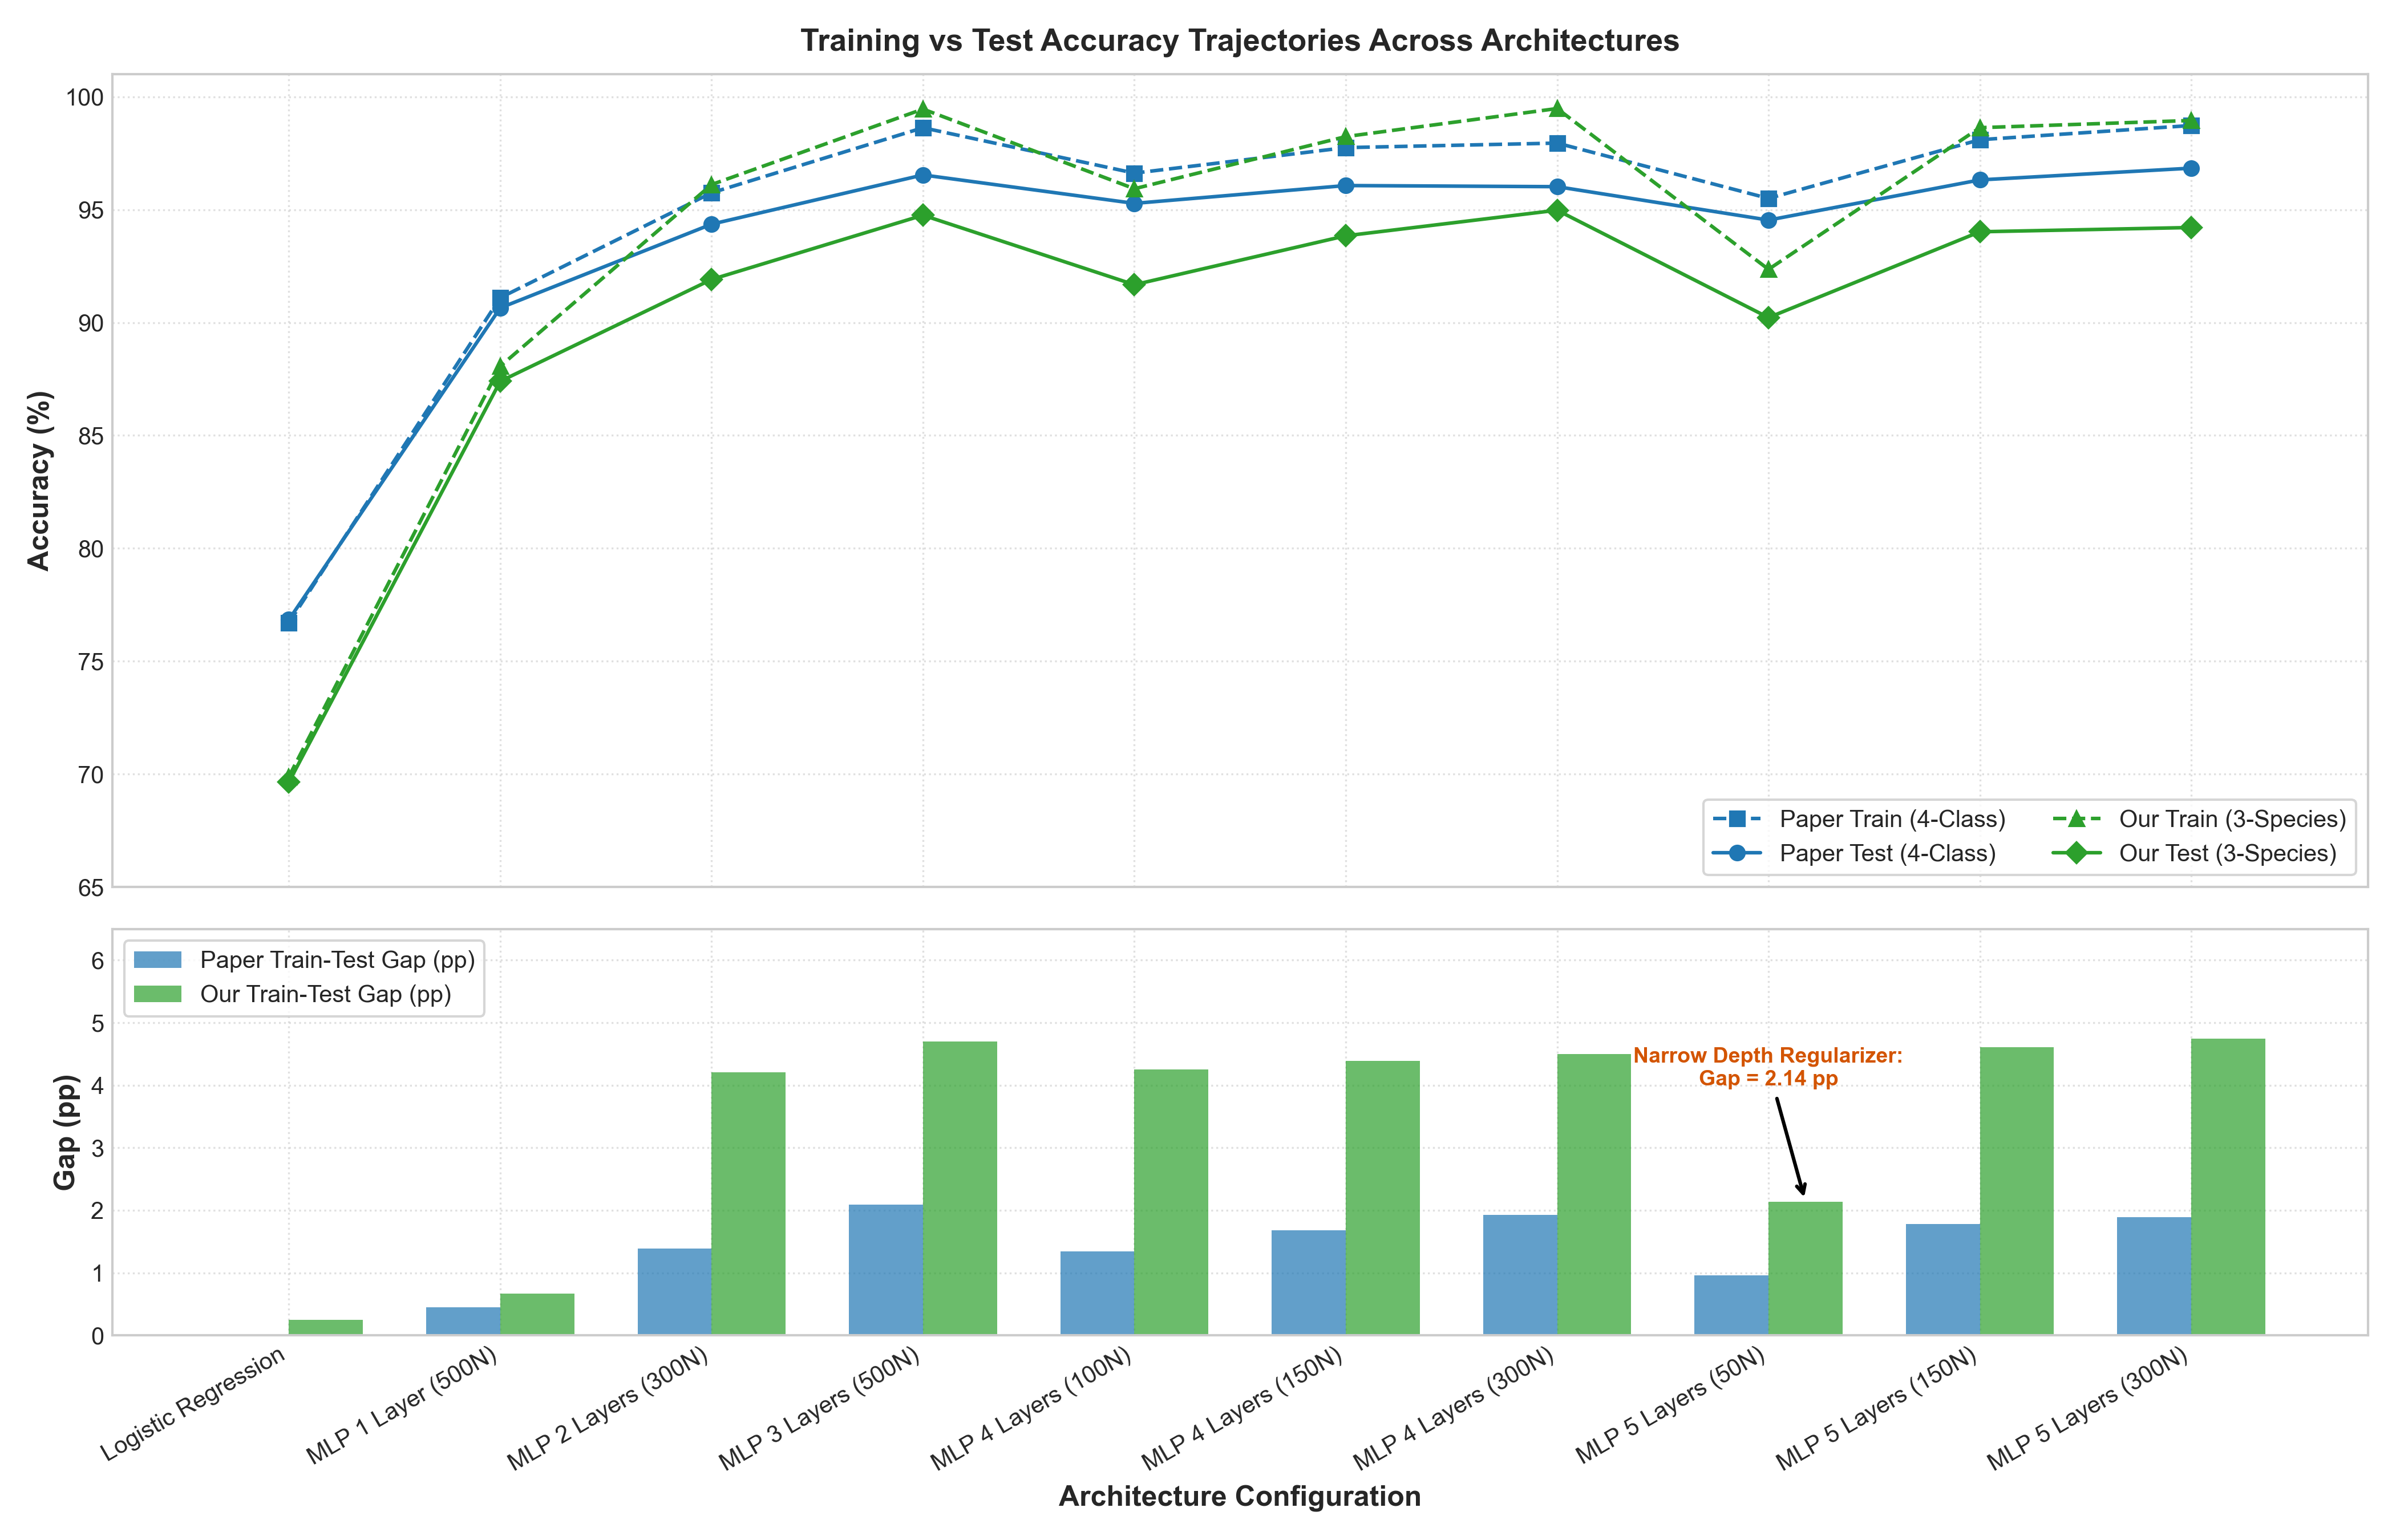
\includegraphics[width=0.96\textwidth]{figs/training_vs_test_accuracy_gap.png}
\caption{Training and test accuracy trajectories across architectures (top) and the corresponding
train--test gap (bottom) for the reported four-class models and the reproduced three-species
models. The narrow five-layer, 50-neuron configuration is annotated.}
\label{fig:gaptraj}
\end{figure*}

\begin{figure*}[!t]
\centering
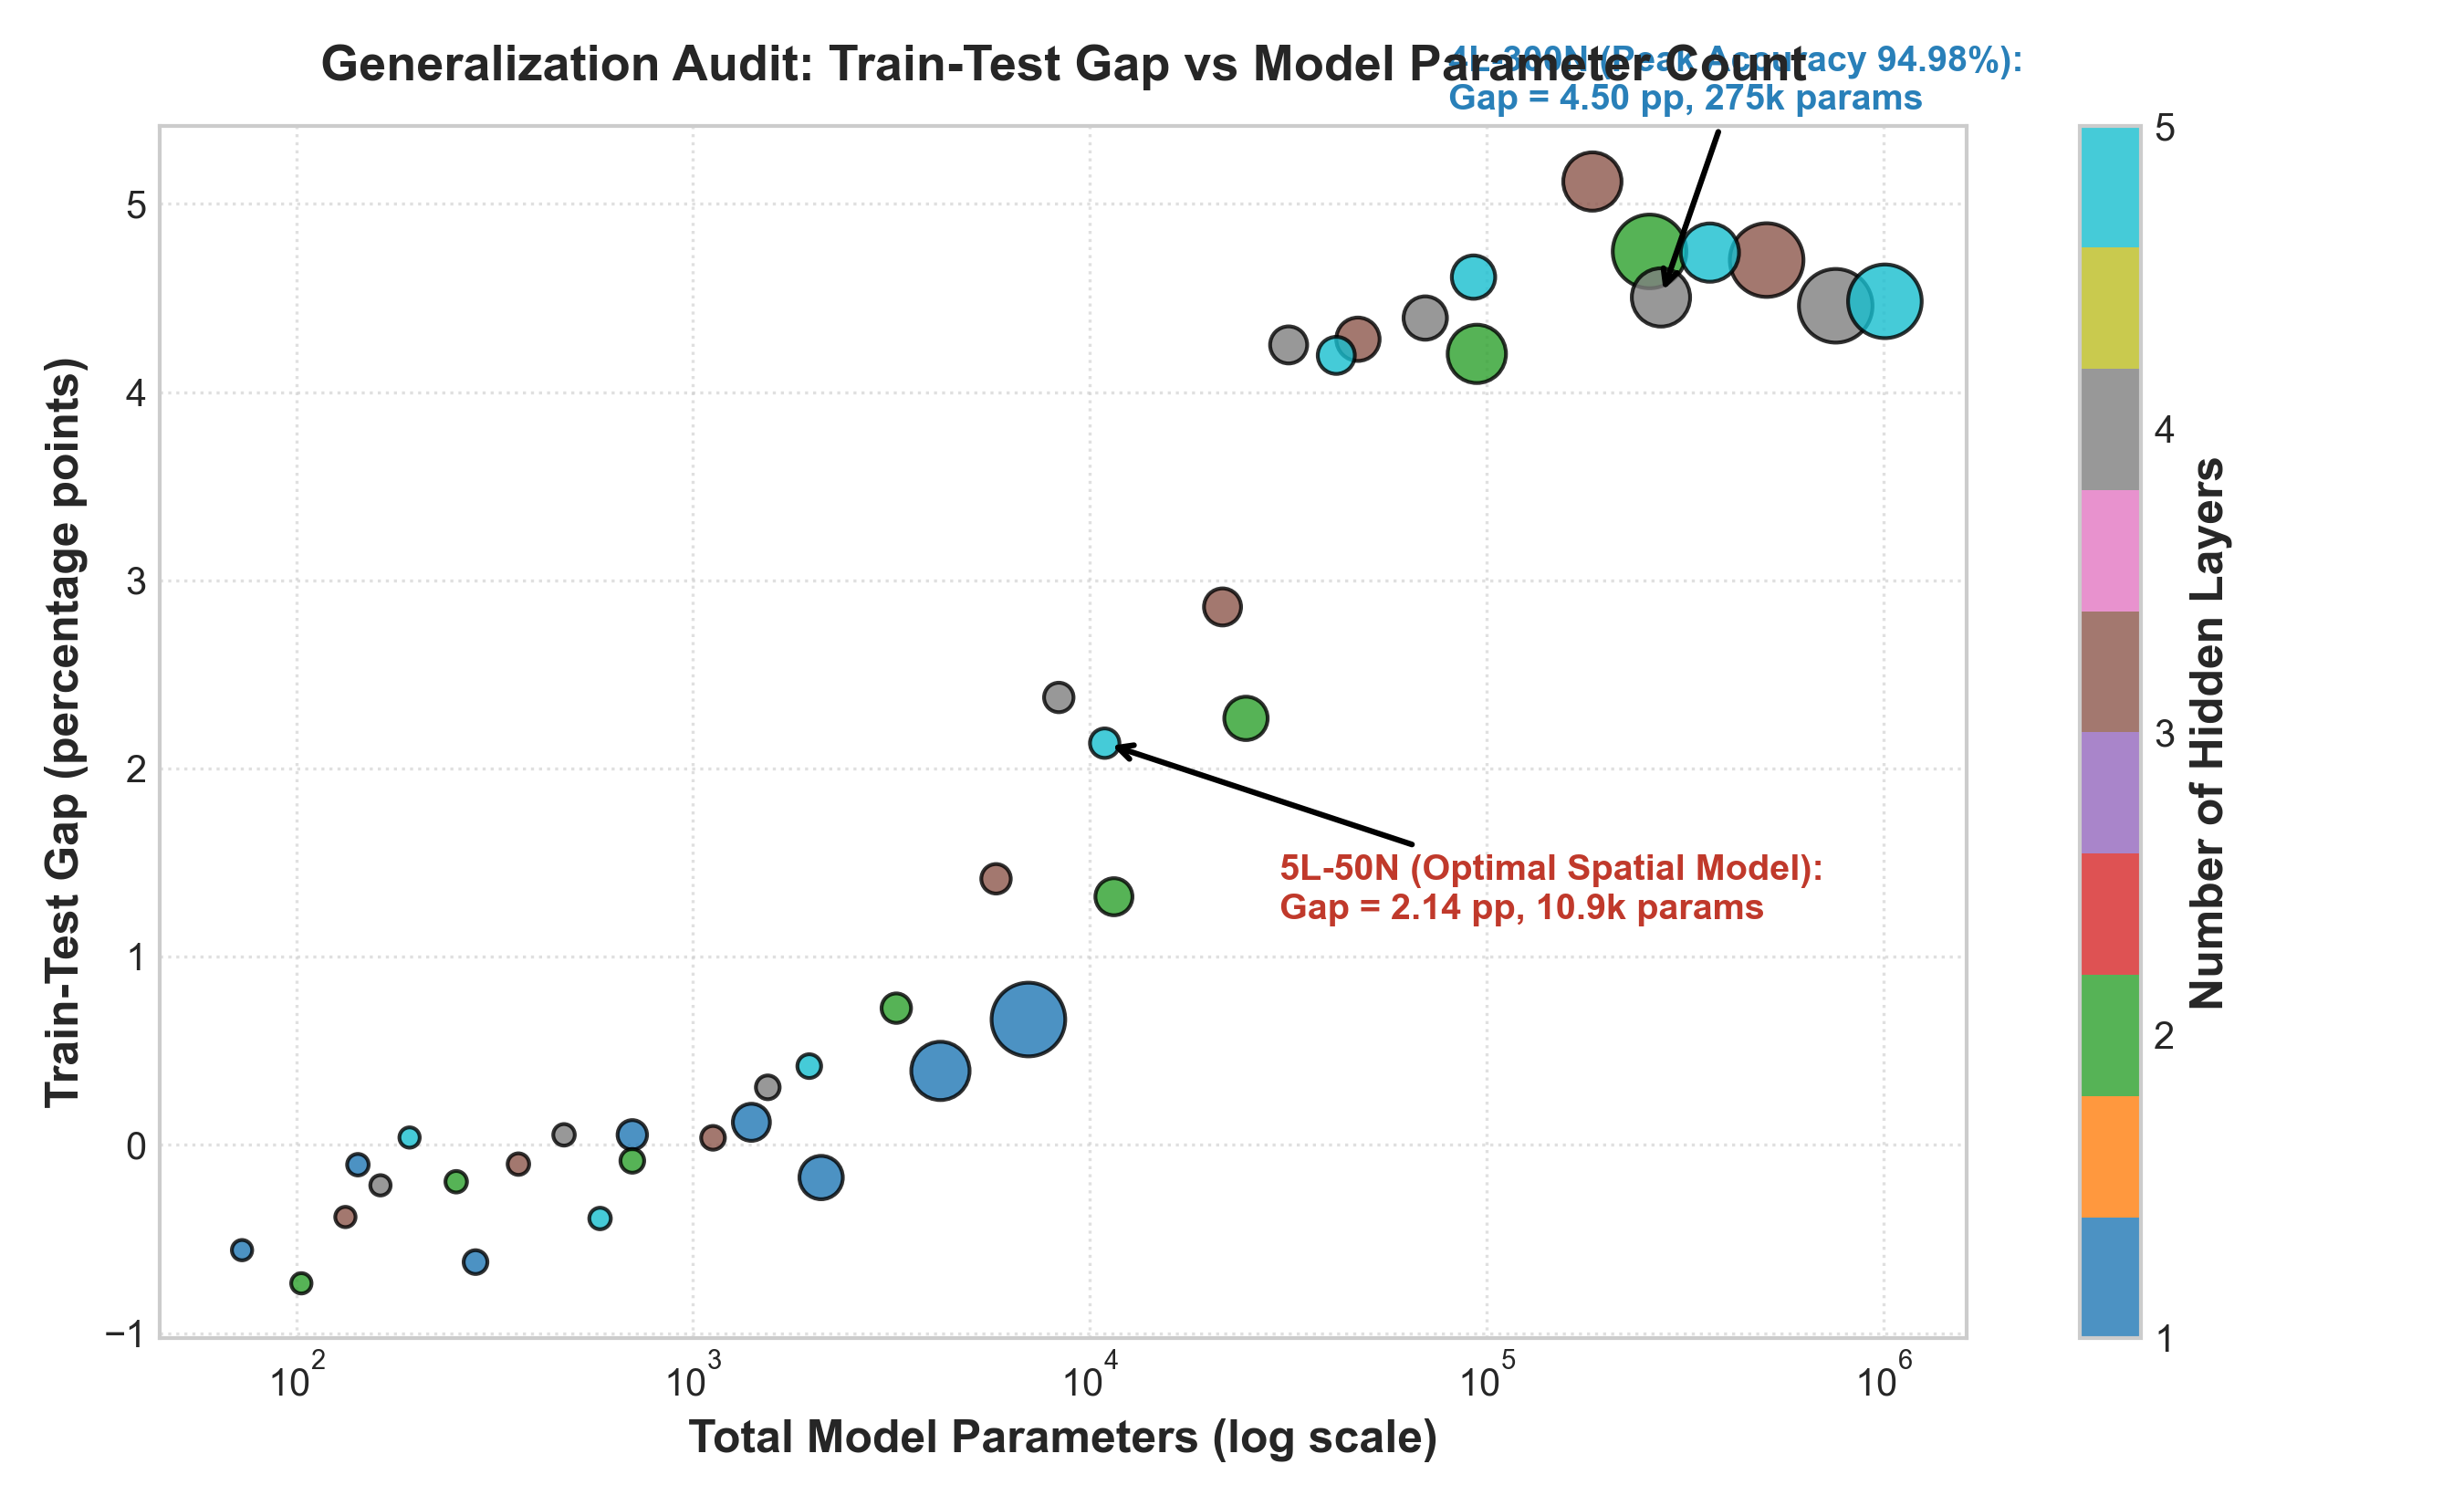
\includegraphics[width=0.96\textwidth]{figs/train_test_gap_analysis.png}
\caption{Train--test gap against total model parameter count (logarithmic scale) for the full
41-model grid, coloured by hidden-layer depth and sized by layer width.}
\label{fig:gapparams}
\end{figure*}

\begin{figure}[!t]
\centering
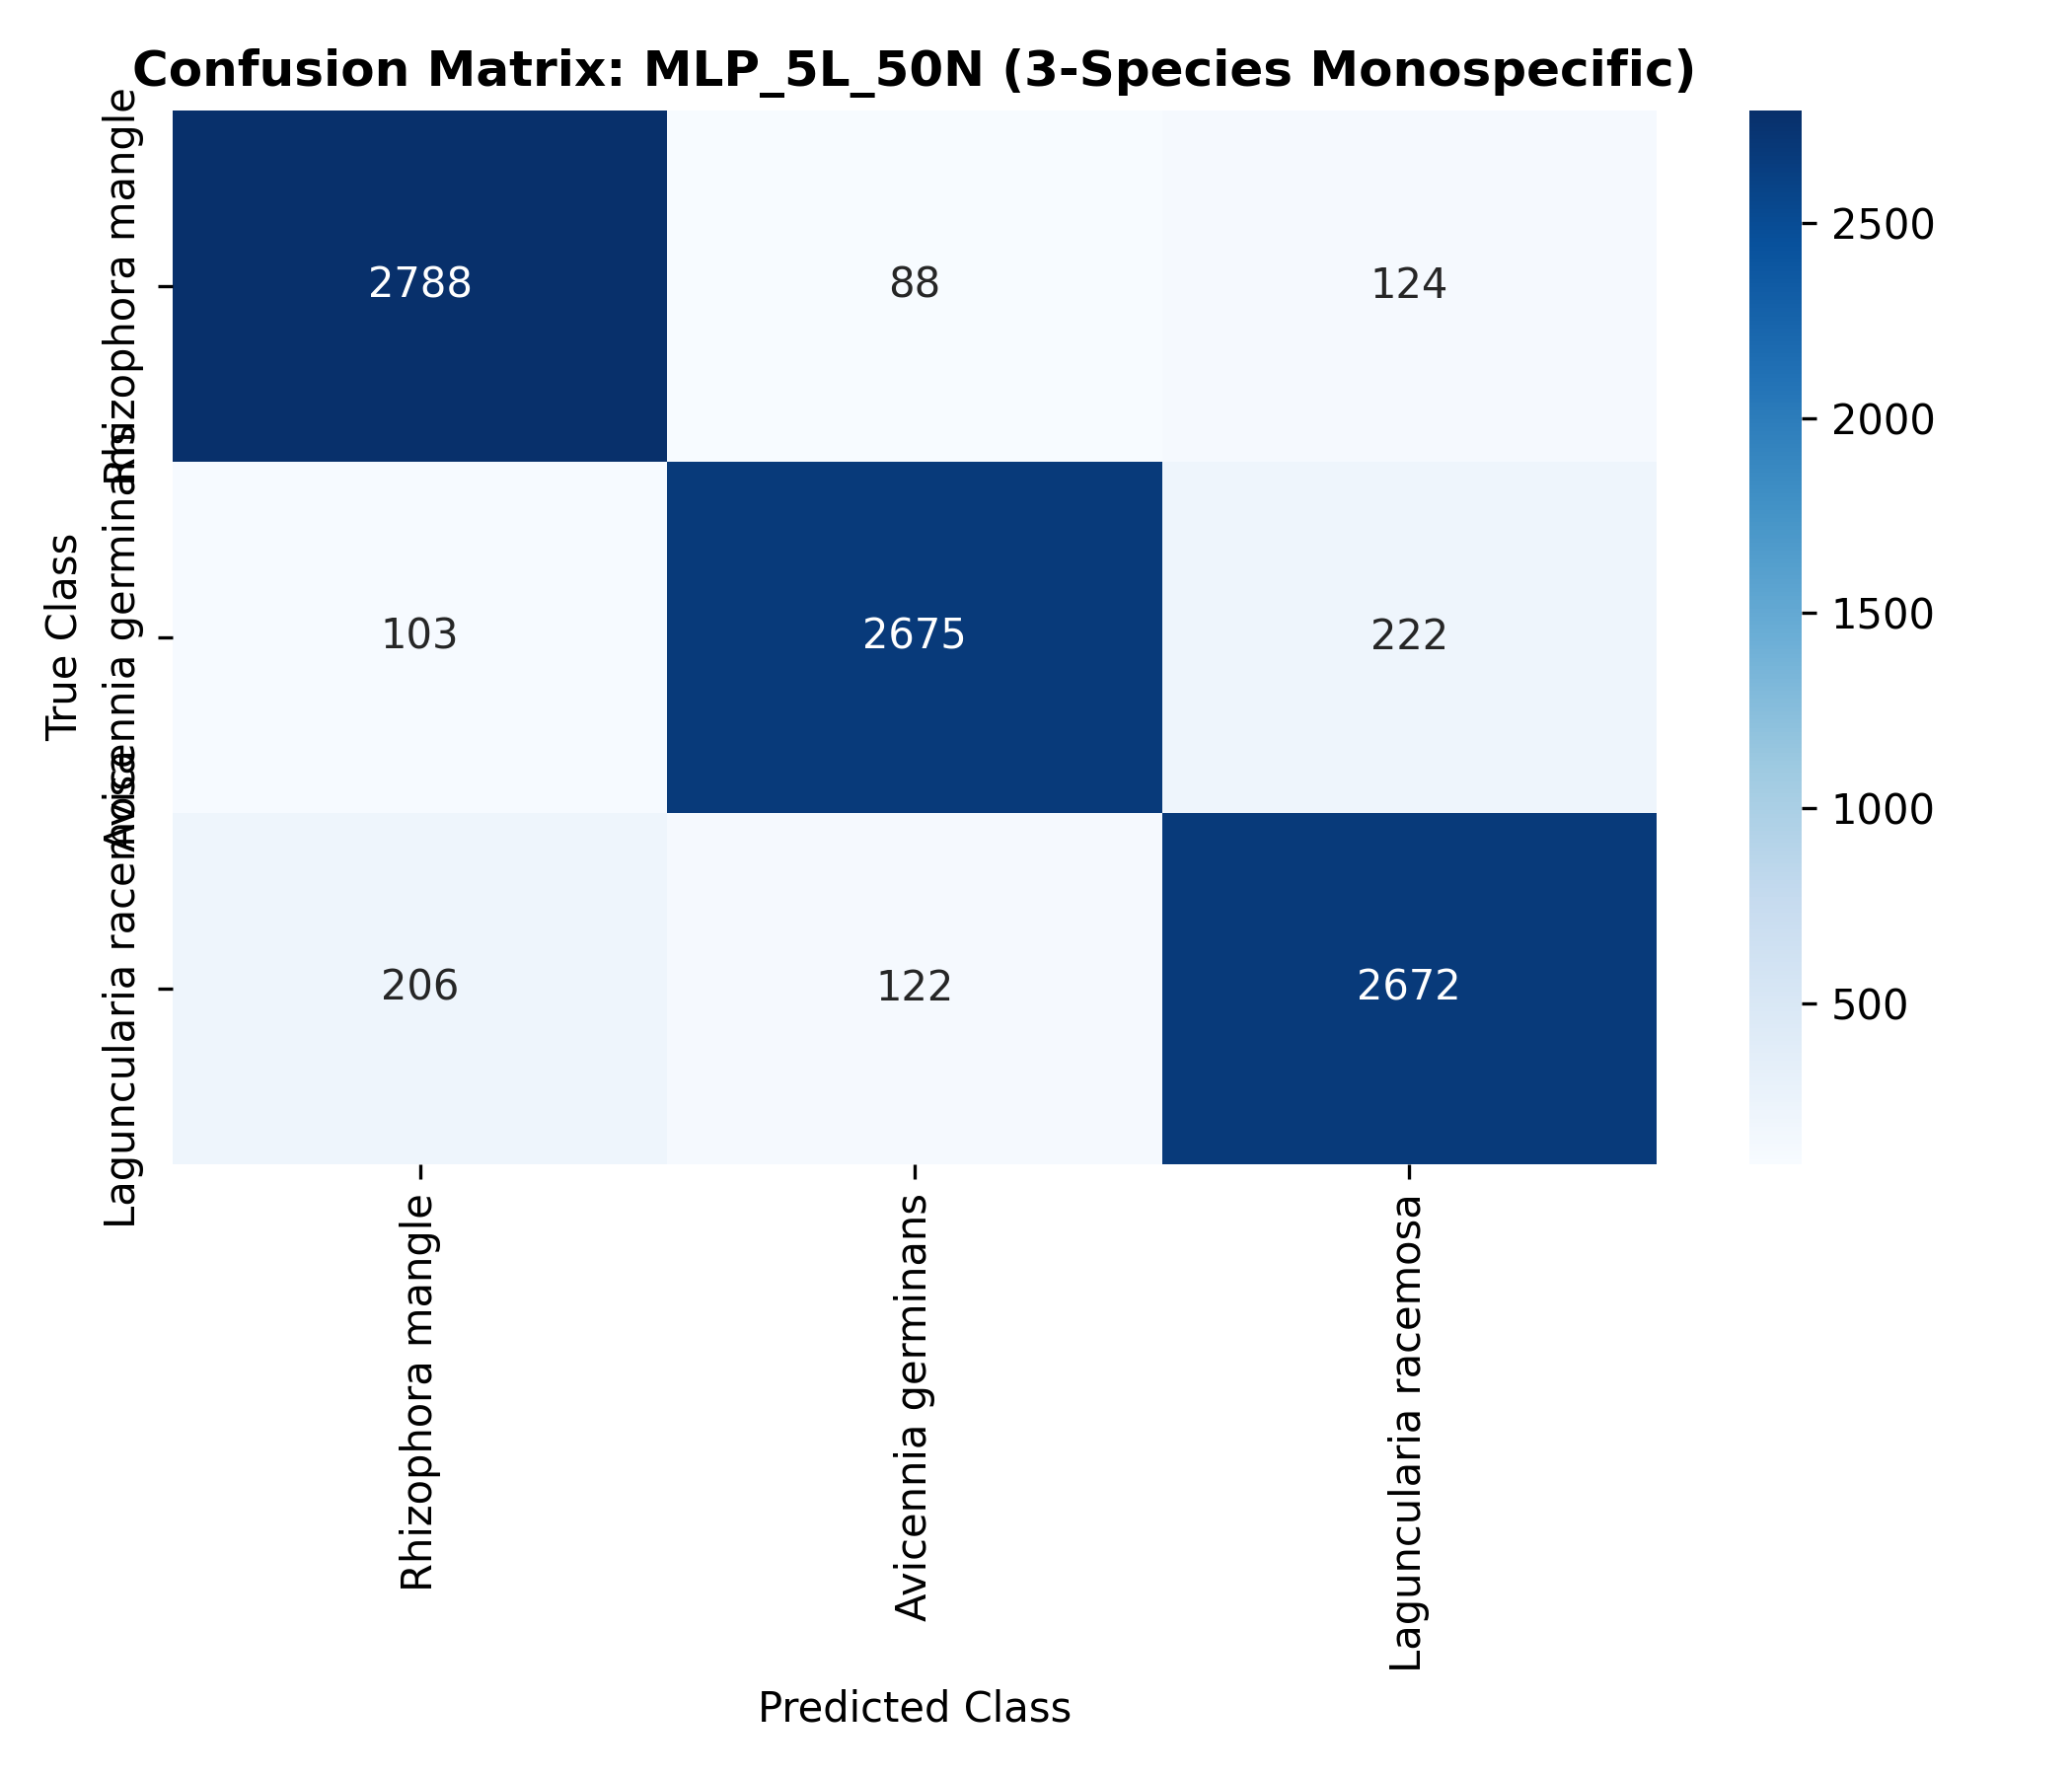
\includegraphics[width=\columnwidth]{figs/three_class_confusion_matrix.png}
\caption{Confusion matrix of the five-layer, 50-neuron model on the 9{,}000-pixel test partition of
the three-species monospecific dataset.}
\label{fig:cm}
\end{figure}

\begin{figure*}[!t]
\centering
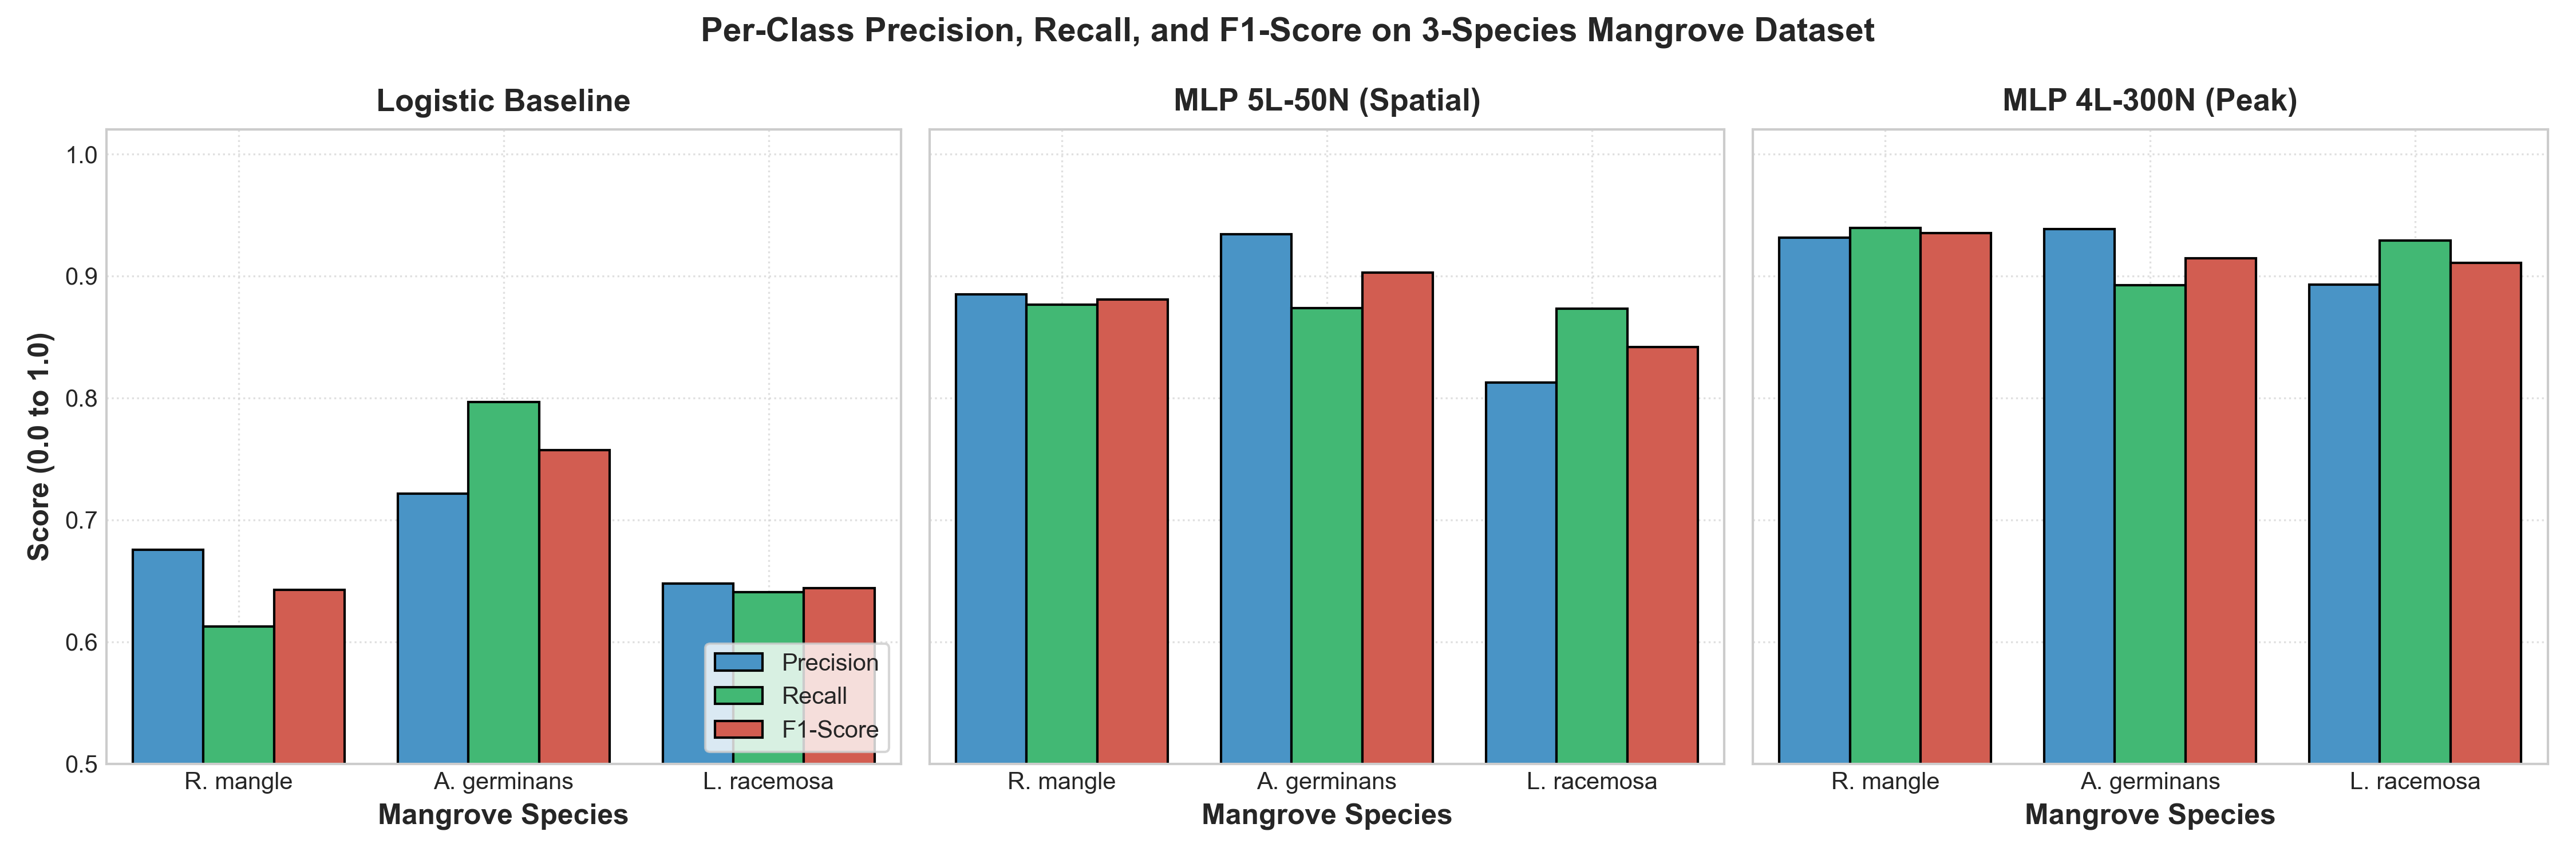
\includegraphics[width=0.96\textwidth]{figs/per_class_prf1_summary.png}
\caption{Per-class precision, recall and $F_1$-score for the logistic baseline, the five-layer
50-neuron model and the four-layer 300-neuron model on the three-species dataset.}
\label{fig:prf1}
\end{figure*}

\subsection{Models test}
\label{sec:results-modelstest}

The spatial evaluation reported in Section~3.3 of \citet{monterrubio2025} is thoroughly described
in the original text but is not reproducible at raster level, because the Sentinel-2 scene
GeoTIFFs, the 3.5\,cm UAV orthophoto and the QGIS species polygons were not deposited. The status
of this component is therefore \evc{DATA-LIMITED}: the methodology is auditable, the outputs are
not. No substitute imagery was obtained and no mask was synthesised.

What the audit preserves is a record of the original authors' reported spatial findings, restated
here as claims of the original study rather than as findings of this reproduction, together with
the spectral evidence in the released data that bears on them. \citet{monterrubio2025} report that,
for the binary models, accuracy exceeded 99\,\% for every architecture yet spatial quality varied
substantially, with the logistic baseline producing extensive salt-and-pepper noise and false
positives over water, and the four-layer, 300-neuron model delineating mangrove boundaries most
cleanly. For the multiclass models, they report that the configuration with the highest test
accuracy suffered spectral confusion between \emph{R.\ mangle} and surrounding water bodies, that
the simpler models overestimated \emph{L.\ racemosa}, and that the five-layer, 50-neuron model was
judged the most reliable for real-world mapping despite its lower test accuracy. At Arroyo Moreno
they report that the models produced plausible predictions without retraining on that site, with
\emph{R.\ mangle} again overestimated in permanently flooded zones while \emph{A.\ germinans} and
\emph{L.\ racemosa} boundaries matched historical field surveys \citep{lopezportillo2002atlas}.
None of these spatial outputs could be independently regenerated or inspected in this reproduction,
and the description above should be read as a summary of the original text, not as an independently
verified result.

Two features of the spectral evidence available in this reproduction are, at least qualitatively,
compatible with two of these reported spatial observations, without constituting independent
verification of either. The reported confusion of \emph{R.\ mangle} with water is qualitatively
consistent with Figs.~\ref{fig:signatures} and \ref{fig:densities}: \emph{R.\ mangle} has the
lowest shortwave infrared reflectance of the three species in the released data and by far the
widest dispersion, so its lower tail overlaps the reflectance region typically occupied by open and
turbid water; the original authors attribute this to the higher moisture content of mangrove canopy.
The reported tendency of simpler models to overestimate \emph{L.\ racemosa} runs in the same
direction as the per-class metrics of Fig.~\ref{fig:prf1}, where that species carries the lowest
precision and the highest recall under the narrow five-layer model on the tabular three-class
problem. These are consistency checks at the level of spectral plausibility, not confirmations of
the spatial maps themselves, which remain outside the reach of this reproduction
(Section~\ref{sec:threats}).


\section{Reproducibility audit findings}
\label{sec:audit}

Table~\ref{tab:audit} consolidates the file-by-file and claim-by-claim audit described in
Section~\ref{sec:methods} into a single reproducibility-status matrix, using the same five-label evidence taxonomy
introduced in Section~\ref{sec:taxonomy}. It is intended as a primary, citable output of this study in its own
right: a reader who wants to know, for a specific component of \citet{monterrubio2025}, whether it
can currently be independently verified, can consult this table directly rather than the discursive
text.

\begin{table*}[!t]
\centering
\caption{Reproducibility audit matrix. ``Available'' records whether the artefact or method detail
is recoverable from the public deposit or the paper text; ``Reproduced'' records whether it was
independently executed or verified in this study. Evidence status follows the taxonomy of
Section~\ref{sec:taxonomy}.}
\label{tab:audit}
\scriptsize
\setlength{\tabcolsep}{2.6pt}
\begin{tabular}{p{2.55cm} p{3.55cm} c c p{2.15cm} p{5.0cm}}
\toprule
\textbf{Component} & \textbf{Required artefact / method} & \textbf{Avail.} & \textbf{Repro.} & \textbf{Evidence status} & \textbf{Limitation} \\
\midrule
Dataset inventory & File-level manifest of the KNB deposit & Yes & Yes & \evc{DATA-DERIVED} & Manifest is limited to what was actually deposited (Sec.~\ref{sec:dataaudit}). \\
Public reflectance CSV & Released 191\,MB CSV, 1{,}605{,}681 rows (\texttt{...LaMancha.csv}) & Yes & Yes & \evc{DATA-DERIVED} & Contains only the three monospecific mangrove species, no background class. \\
Spectral bands (10) & B2--B12 surface reflectance, pre-resampled & Yes & Yes & \evc{PAPER-SPECIFIED} / \evc{DATA-DERIVED} & --- \\
Preprocessing (StandardScaler) & Fit-on-train, transform-train-and-test & Partial & Yes (this study) & \evc{PAPER-SPECIFIED} (formula) / \evc{NOT AVAILABLE} (fit order in original) & Original fit-before/after-split order not stated; this study's own procedure is documented but is not evidence about the original implementation. \\
One-way ANOVA & Per-band $F$-test, 3 species & Yes & Yes & \evc{DATA-DERIVED} & Large-$n$ significance; no effect sizes computed (Sec.~\ref{sec:results-stats}). \\
Tukey HSD & 30 pairwise post-hoc contrasts & Yes & Yes & \evc{DATA-DERIVED} & Same non-independence caveat as ANOVA. \\
Spectral signature curves & Mean $\pm$ SD reflectance per band & Yes & Yes & \evc{DATA-DERIVED} & --- \\
Band correlation analysis & Pearson correlation matrix & Yes & Yes & \evc{DATA-DERIVED} & --- \\
41-model MLP grid & Logistic $+$ 1--5 layers $\times$ 8 widths & Yes (arch.\ spec.) & Yes, on 3-class data & \evc{PAPER-SPECIFIED} (grid) / \evc{DATA-DERIVED} (results) & Trained on 3-class, not on the original 4-class or binary label space. \\
Binary classification (60k px) & Mangrove vs non-mangrove pixels & No & No & \evc{DATA-LIMITED} & Non-mangrove pixels not deposited; not attempted. \\
Four-class classification (40k px) & 3 species $+$ non-mangrove & No & No & \evc{DATA-LIMITED} & Non-mangrove pixels not deposited; not attempted. \\
Non-mangrove samples & Rainforest, crops, water, urban, dunes, wetlands & No & No & \evc{DATA-LIMITED} & Not deposited; not substituted or fabricated (Sec.~\ref{sec:intro}). \\
UAV orthophoto & 3.5\,cm GeoTIFF, La Mancha & No & No & \evc{DATA-LIMITED} & Not deposited. \\
QGIS species masks & Vector polygons, 3 species $+$ mixed & No & No & \evc{DATA-LIMITED} & Not deposited. \\
Sentinel-2 scene GeoTIFFs & Full-scene rasters, La Mancha \& Arroyo Moreno & No & No & \evc{DATA-LIMITED} & Not deposited. \\
Spatial mapping (Figs.~7--9) & Pixel-wise prediction over scene rasters & No & No & \evc{DATA-LIMITED} & Requires the scene GeoTIFFs above. \\
Spatial validation (Fig.~10) & Cross-site prediction at Arroyo Moreno & No & No & \evc{DATA-LIMITED} & Requires the scene GeoTIFFs above. \\
Original hyperparameters & Learning rate, batch size, epochs & No & N/A & \evc{NOT AVAILABLE} & Not stated in text; this study used documented \evc{IMPLEMENTATION ASSUMPTION} values (Sec.~\ref{sec:methods-mlp}). \\
Original random seed(s) & Sampling, split, initialisation seeds & No & N/A & \evc{NOT AVAILABLE} & This study fixed seed 42 throughout; not the original authors' value(s). \\
Cross-site / cross-scene split & Scene- or site-blocked train/test partition & No & No & \evc{NOT AVAILABLE} & Neither study reports a spatially blocked evaluation; risk discussed in Section~\ref{sec:threats}. \\
\bottomrule
\end{tabular}
\end{table*}

\section{Threats to validity}
\label{sec:threats}

This section makes explicit the limitations that constrain what can legitimately be claimed from
the results in Section~\ref{sec:results}, organised into internal, statistical, external and reproducibility
validity. None of these limitations is newly discovered here; they follow directly from the
evidence audit in Sections~2 and \ref{sec:audit} and are collected here so that a reader can assess,
in one place, the conditions under which the reported numbers should be interpreted.

\subsection{Internal validity}
\label{sec:threats-internal}

The original learning rate, batch size, epoch count, weight-initialisation scheme and random seeds
are \evc{NOT AVAILABLE}, and the documented \evc{IMPLEMENTATION ASSUMPTION} values used here
($\alpha=0.001$, batch size 256, 30 epochs, seed 42, PyTorch Kaiming-uniform initialisation) are not
known to match the original implementation's. The original work cites a Keras/TensorFlow reference
\citep{chollet2021}, whose default Glorot-uniform initialisation differs from the PyTorch default
used here, and framework-level differences in optimiser numerics, data-loader shuffling and
floating-point behaviour are a further source of internal-validity uncertainty. The preprocessing
order (whether standardisation was fit before or after the train/test split in the original study)
is not stated in the text and is \evc{NOT AVAILABLE}; this reproduction fits the scaler on the
training partition only, which is stated as this study's own documented choice and not as a
recovered fact about the original pipeline. The train/test split itself is performed at the pixel
level with stratification by class label but without blocking by scene, acquisition date or spatial
location, which creates the possibility, discussed under statistical validity below, that
information from a given location leaks between partitions. All of these are threats to the
internal validity of the numerical accuracies reported in Tables~\ref{tab:ours}--\ref{tab:diff}, in
the sense that a different, equally defensible set of implementation choices could plausibly
produce different accuracy values on the same data.

\subsection{Statistical validity}
\label{sec:threats-statistical}

The pixel-level observations that enter the ANOVA, the Tukey HSD tests and the classification
accuracies are not statistically independent: multiple pixels are drawn from the same monospecific
polygon, the same polygon is imaged repeatedly across 147 temporally correlated Sentinel-2
acquisitions of the same two sites, and neighbouring pixels within a scene are spatially
autocorrelated. Classical ANOVA and the accuracy estimates reported here assume independent and
identically distributed observations; that assumption is not satisfied by construction, so the very
small $p$-values obtained ($p<10^{-10}$ for every band) reflect both the underlying spectral
separation and the large, non-independent sample size, and should not be interpreted as evidence of
an unusually large effect. For the same reason, the classification accuracies in
Table~\ref{tab:ours} are best interpreted as performance under a stratified random pixel-level
holdout on this specific multi-temporal pixel pool, rather than as an unbiased estimate of accuracy
on genuinely independent, unseen locations or dates. No multi-seed replication was performed, so no
variance or confidence interval is available for any reported accuracy or train--test gap
[AUTHOR INPUT REQUIRED: multi-seed runs would allow this uncertainty to be quantified].

\subsection{External validity}
\label{sec:threats-external}

All results, in both the original study and this reproduction, come from a single study area
(La Mancha, with an out-of-sample application at Arroyo Moreno reported only by the original
authors and not independently verified here), a single sensor (Sentinel-2 L1C), a single
acquisition period (2015--2021) and three mangrove species specific to the Gulf of Mexico coast of
Veracruz. Neither the original study nor this reproduction establishes that the reported
architectural or spectral-separability patterns transfer to other mangrove-forming species,
other sensors, other geographic regions, or other combinations of monospecific versus mixed stands.
Claims in this manuscript are accordingly restricted to the study area and species evaluated, and no
general claim about mangrove species classification is intended.

\subsection{Reproducibility validity}
\label{sec:threats-repro}

The non-mangrove background pixels, the subsampled 60{,}000-pixel binary and 40{,}000-pixel
four-class training sets, the UAV orthophoto, the QGIS vector masks and the Sentinel-2 scene
GeoTIFFs described in the original methodology are \evc{DATA-LIMITED}: described in the text but
absent from the public deposit (Table~\ref{tab:audit}). As a direct consequence, the original
binary classification experiment, the original four-class classification experiment, and the
spatial mapping and cross-site validation of Figs.~7--10 cannot be independently reproduced from
public evidence, and are not reproduced in this manuscript. The original specification is also
incomplete on several points needed for exact reproduction
(Section~\ref{sec:threats-internal} above),
which independently limits reproducibility even where the relevant data are available. These
limitations are structural properties of the public record for this study, not shortcomings of the
reproduction effort, and they define the boundary of what any independent audit of this study can
currently establish.

\section{Discussion}
\label{sec:discussion}

This study indicates that the statistical foundation of \citet{monterrubio2025} can be reproduced
from the publicly deposited data, and that its principal architectural interpretation is not
contradicted by an independently computed, complementary measure, while its headline accuracy
figures remain outside what the public record supports. This is a scope statement about what has
and has not been independently verified, not a ranking of the two studies; the distinction matters
because the three components carry different evidential weight for a reader deciding how much to
rely on the original method.

The exploratory result was reproduced from the released data. Every band separates the three
species at $p<10^{-10}$ and all thirty pairwise Tukey contrasts are significant, providing evidence
consistent with the premise that Sentinel-2 reflectance carries species-level information in
Veracruz mangroves, subject to the statistical-validity caveats of Section~\ref{sec:threats}
regarding pixel non-independence and effect size. The practical consequence emphasised by the
original authors, that multispectral data can be used directly to identify mangrove distribution
without additional processing such as vegetation indices, is not contradicted by the 94.98\,\%
three-species accuracy obtained here from raw standardised reflectance alone on a different
(three-class, not four-class) class space.

The architectural interpretation is examined here through a different instrument than the one the
original authors used. Their preference for the five-layer, 50-neuron model rested on visual
inspection of predicted maps, which are not available for this reproduction. The train--test gap
analysis in Section~\ref{sec:gap} offers a measurable, though indirect, complement to that judgement: at
approximately 10{,}800 parameters (Table~\ref{tab:ours}; see the parameter-count note in
Section~\ref{sec:gap}) the model shows a gap of 2.14 percentage points where models of comparable depth and
greater width show gaps of 4.4 to 4.7 points. This pattern is consistent with, rather than proof of,
the interpretation offered by the original authors that restricting neurons per layer may limit
overfitting to spectral noise \citep{hagan2014}; it is based on a single seed and ten of the
forty-one configurations, and no controlled experiment isolating width from depth, sample size or
training duration was performed. The pattern also illustrates a methodological point of wider
relevance: in operational remote sensing, where the deliverable is a map rather than a confusion
matrix, model selection on test accuracy alone carries risk, and capacity diagnostics of the kind
computed here may be a useful, low-cost complement to spatial evaluation where the latter is
unavailable \citep{kumaraperumal2022,chowdhury2024}.

The headline accuracies of the original binary and four-class experiments could not be reproduced,
and the reason is structural rather than a matter of implementation effort. The deposited file
contains only monospecific mangrove pixels; the non-mangrove background class described in Section~2.1
of the original article, sampled from rainforest, crops, water, urban areas, dunes and other
wetlands, was not released. Both published experiments depend on it --- one of two classes in the
binary task and one of four in the multiclass task --- so neither could be rebuilt without either
obtaining the missing data from the original authors or fabricating a substitute, both of which are
outside the scope of this study. The $-3.09$ percentage point mean offset between the reported
four-class accuracies and the three-species accuracies obtained here is, accordingly, attributable
to a different class space, with an additional non-mangrove class and a different chance baseline
(25\,\% against 33.3\,\%), and is shown in Table~\ref{tab:diff} and Fig.~\ref{fig:compare} for
audit transparency rather than as a performance comparison. Stating that this reproduction performed
worse, or better, than the original study would not be supported by the evidence available.

Several secondary sources of divergence between the two studies remain unresolved and are recorded
as such rather than adjudicated. The learning rate, batch size, epoch count and random seeds are
absent from the original text, and variation in these quantities can plausibly move test accuracy
by more than a percentage point; the values adopted here are documented but are not known to match
the original authors'. The framework differs, Keras-style Glorot-uniform initialisation against
PyTorch Kaiming-uniform, which is a further obstacle to numerical agreement. The original article
also does not state whether the 70/30 split was stratified or whether pixels were partitioned across
the 147 acquisitions; as set out in Section~\ref{sec:threats}, unblocked pixel-level splitting over
a multi-temporal stack raises the possibility that the same ground location, imaged on different
dates, appears in both partitions of either study, which would be expected to inflate pixel-level
test accuracy relative to genuine out-of-scene generalisation. This is raised as an unverified
structural risk that applies to the splitting procedure described in the original text and to the
splitting procedure used in this reproduction alike, not as a finding that leakage occurred in
either case, which the available information is insufficient to establish.

Two minor inconsistencies were identified in the original text during the audit and are recorded
for completeness. The description in Section~3.3 attributes a training score of 0.9775 and a test
score of 0.9607 to a one-hidden-layer model with 150 neurons, whereas the caption of Fig.~9 and the
surrounding context identify this configuration as a four-hidden-layer model; the figure caption
appears to be correct. In addition, all numerical results are presented through bar charts and
spatial maps, with only selected models quoted in the text, so no complete tabular record of the
41-model grid exists in the published article. Both observations are offered as reproducibility
notes rather than as errors of substance, and neither affects the study's conclusions.

\section{Recommendations for reproducible ecological machine learning}
\label{sec:recommendations}

The findings above motivate a small set of concrete recommendations, addressed primarily to future
data deposition and evaluation practice in this subfield rather than to the original authors
specifically.

\textbf{Deposition completeness.} The authors deposited a substantial and well-documented dataset,
and it is precisely because the monospecific pixels were released that the statistical analysis and
the architectural scaling behaviour could be examined at all. Extending the same deposit to the
non-mangrove background table, to the two subsampled datasets actually used for training, and to the
random seeds and optimiser settings would allow the published accuracies to be independently
verified at comparatively low additional cost. Where scene GeoTIFFs are too large to archive
routinely, depositing the scene identifiers and acquisition dates, together with the vector masks,
would allow an independent party to rebuild the spatial test from the Copernicus archive.

\textbf{Spatially or temporally blocked evaluation.} The pixel-level-leakage risk described in
Section~\ref{sec:threats} could be addressed at the design stage by partitioning pixels by scene or
by spatial block rather than at random, and by reporting accuracy on a held-out acquisition or a
held-out spatial region. Given the modifiable areal unit problem and its implications for mangrove
extent estimates \citep{jelinski1996}, an evaluation protocol that separates spatial from temporal
generalisation would strengthen claims of transferability such as the Arroyo Moreno test reported by
the original authors.

\textbf{Multi-seed reporting.} Neither the original study nor this reproduction reports results
from more than a single run per configuration. Reporting mean and spread across several random
seeds, particularly for the architectures singled out for their generalisation behaviour, would
allow a reader to judge whether differences such as the 2.14-percentage-point train--test gap of the
five-layer, 50-neuron model in this reproduction are stable or fall within run-to-run variability
[AUTHOR INPUT REQUIRED: multi-seed results for this reproduction, if produced in a future revision].

\textbf{Effect sizes alongside significance tests.} Given the very large and non-independent pixel
counts involved, reporting a standardised effect size (for example, $\eta^2$ per band) alongside
each ANOVA result would let readers separate statistical detectability from ecological or spectral
importance [AUTHOR INPUT REQUIRED: effect-size computation, not performed in the present
reproduction].

\textbf{Context-aware architectures.} The direction of future work indicated by the original
authors --- moving beyond pixel-wise perceptrons to segmentation architectures such as U-Net that
incorporate spatial context alongside spectral response --- is consistent with the error structure
documented here. The residual confusions reported by the original authors and reflected in the
tabular per-class metrics of this reproduction, the confusion of \emph{R.\ mangle} with water in
flooded zones and the overestimation of \emph{L.\ racemosa}, are spatially organised phenomena that
a classifier operating on one pixel at a time cannot, by construction, resolve. Reproducible
evaluation of such context-aware models will depend on the deposition practices described above.

\section{Conclusions}
\label{sec:conclusions}

This study conducted an independent reproduction and reproducibility audit of
\citet{monterrubio2025}, applying a five-label evidence taxonomy to every element of the original
methodology. The scope of this conclusion is limited to what the evidence assembled in
Sections~3--\ref{sec:threats} supports; it is not a re-adjudication of the original study's own
conclusions, which this work is not positioned to overturn.

\textbf{What was reproduced.} The exploratory and statistical analysis was reproduced from the
publicly deposited data: one-way ANOVA on each of the ten Sentinel-2 bands and all thirty pairwise
Tukey HSD contrasts return significant differences between \emph{R.\ mangle}, \emph{A.\ germinans}
and \emph{L.\ racemosa} ($p<10^{-10}$ and $p<0.001$ respectively), consistent with the original
study's Fig.~4, subject to the pixel-non-independence caveat of Section~\ref{sec:threats}. The
41-configuration architectural grid was re-implemented and trained on a balanced 30{,}000-pixel
three-species dataset derived from the deposited file under a stratified pixel-level holdout,
yielding test accuracies from 69.64\,\% for the logistic baseline to 94.98\,\% for the four-layer,
300-neuron model. This indicates that, under this experimental design, three co-occurring mangrove
species are separable at better than 94\,\% from raw standardised reflectance without vegetation
indices.

\textbf{What was examined, but not proved.} A train--test gap analysis found that the five-layer,
50-neuron configuration the original authors selected for spatial mapping shows a gap of 2.14
percentage points at approximately 10{,}800 parameters, smaller than the 4.4--4.7 point gaps of
wider models of similar depth. This single-seed, ten-configuration observation is consistent with,
and offers a quantitative complement to, the original authors' qualitative argument that narrower
layers may limit overfitting; it does not, on its own, establish a causal regularisation mechanism,
and it was not tested through a controlled capacity experiment or multiple seeds.

\textbf{What was not, and could not be, reproduced.} The published binary (60{,}000-pixel) and
four-class (40{,}000-pixel) accuracies, and the full-scene spatial predictions of Figs.~7--10, are
not reproducible from the public record, because the non-mangrove background pixels, the two
subsampled training datasets, the UAV orthophoto, the QGIS vector masks and the Sentinel-2 scene
GeoTIFFs were not deposited (Table~\ref{tab:audit}). These values are reported in this manuscript as
reference benchmarks, shown alongside the three-species results for audit transparency only. The
mean offset of $-3.09$ percentage points between them and the three-species results obtained here is
attributable to a different class space and a different chance baseline, and does not constitute a
comparison of model quality in either direction.

\textbf{Limitations affecting interpretation.} The undocumented original hyperparameters and random
seeds, the framework difference between the likely Keras/TensorFlow original implementation and the
PyTorch implementation used here, the unblocked pixel-level train/test split common to both studies,
the single-seed design of this reproduction, and the restriction of both studies to one study area,
one sensor and three species together bound what can be claimed from the results
(Section~\ref{sec:threats}).

\textbf{Recommendation for future work.} Readers seeking to build on either study should treat the
reported accuracies as specific to the stratified random pixel-level holdout, the study area and the
acquisition period evaluated, and should prioritise, where resources allow, spatially or temporally
blocked evaluation splits, multi-seed replication, and deposition of the background-class data
needed to close the binary and four-class reproduction gap identified here.

All reproduction code, notebooks and generated results supporting this audit are released publicly
(see the Data and code availability statement at the end of this article) so that the audit itself
remains open to independent scrutiny.

\section*{Description of author's responsibilities}

\noindent Bala Sudalaimuthu: Conceptualisation, methodology, software, formal analysis, data
curation, visualisation, writing --- original draft, writing --- review and editing.

\section*{Declaration of competing interest}

The author declares no competing financial interests or personal relationships that could have
appeared to influence the work reported in this paper. This study is an independent reproduction
and was conducted without the involvement of the authors of the original article.

\section*{Acknowledgements}

The author thanks Monterrubio-Mart\'inez et al.\ for depositing the monospecific Sentinel-2
reflectance dataset in the Knowledge Network for Biocomplexity, without which none of the
verification reported here would have been possible, and acknowledges the European Space Agency and
the Copernicus programme for open access to Sentinel-2 data.

\section*{Data and code availability}
\label{sec:data}

\textbf{Original dataset (publicly available).} The dataset analysed by \citet{monterrubio2025} and
audited in this study is openly available from the Knowledge Network for Biocomplexity (KNB) under
package identifier \texttt{doi:10.5063/F1FN14P1}
(\url{https://knb.ecoinformatics.org/view/doi:10.5063/F1FN14P1}), titled ``Sentinel-2 satellite
reflectance of monospecific mangrove forests (\emph{Rhizophora mangle}, \emph{Avicennia germinans}
and \emph{Laguncularia racemosa}) at 10\,m spatial resolution in La Mancha, Veracruz, Mexico from
2015--2021'', published 2024-11-07 under a Creative Commons Attribution 4.0 International
(CC-BY-4.0) licence. It comprises the reflectance CSV
(\texttt{DataBase\_Sentinel\_2\_Mangrove\_LaMancha.csv}, 191\,MB, 1{,}605{,}681 rows) and an
Ecological Metadata Language (EML v2.2.0) XML descriptor.

\textbf{Original artefacts not publicly available.} The non-mangrove background reflectance table,
the subsampled 60{,}000-pixel binary and 40{,}000-pixel four-class training sets, the original
authors' source code and model checkpoints, the 3.5\,cm UAV orthophoto, the QGIS vector masks, and
the Sentinel-2 scene GeoTIFFs for La Mancha and Arroyo Moreno were not found in the KNB deposit and
are, to the knowledge of this study, not otherwise publicly released (Table~\ref{tab:audit}).

\textbf{Reproduction code, notebooks and results.} All code, Jupyter notebooks, generated result
tables and figure-generation scripts produced for this independent reproduction are released
publicly at \url{https://github.com/notfawkes/Mangroves-Blue-Carbon.git}. The repository includes
eight executed notebooks covering the dataset audit, the statistical reproduction, the MLP
re-implementation and the paper-versus-reproduction comparison; the modular source code
(\texttt{src/config.py}, \texttt{src/data/loader.py}, \texttt{src/models/mlp.py},
\texttt{src/stats/anova\_tukey.py}, \texttt{src/training/trainer.py}); the generated result tables
(\texttt{results/models/three\_class\_mangrove\_results.csv},
\texttt{results/architecture\_comparison.csv}, \texttt{results/anova\_results.csv},
\texttt{results/tukey\_results.csv}); the twelve figures reproduced in this manuscript
(\texttt{results/figures/}); the discrepancy-audit documents underlying Sections~2,
\ref{sec:audit} and \ref{sec:threats} (\texttt{results/PAPER\_VS\_REPRODUCTION.md},
\texttt{SPATIAL\_REPRODUCTION\_STATUS.md}); and a small unit-test suite
(\texttt{tests/test\_reproduction.py}).

\textbf{Computational environment.} The reproduction was executed in Python 3.9.6 with PyTorch
2.8.0 (Apple Silicon, Metal Performance Shaders backend), scikit-learn 1.6.1, SciPy 1.13.1,
statsmodels 0.14.6, pandas 2.3.3 and NumPy 2.0.2, as against the paper's stated Python 3.8.13 and
scikit-learn 1.2.1 with an implied Keras/TensorFlow backend \citep{chollet2021}. Exact package
versions are pinned in the repository's environment specification.

\begin{thebibliography}{99}
\footnotesize

\bibitem[Chollet(2021)]{chollet2021}
Chollet, F., 2021. Deep Learning with Python, 2nd ed. Manning Publications.

\bibitem[Chopade et al.(2023)]{chopade2023}
Chopade, M.R., Mahajan, S., Chaube, N., 2023. Assessment of land use, land cover change in the
mangrove forest of Ghogha area, Gulf of Khambhat, Gujarat. Expert Syst. Appl. 212.
\url{https://doi.org/10.1016/j.eswa.2022.118839}.

\bibitem[Chowdhury(2024)]{chowdhury2024}
Chowdhury, M.S., 2024. Comparison of accuracy and reliability of random forest, support vector
machine, artificial neural network and maximum likelihood method in land use/cover classification
of urban setting. Environ. Challeng. 14, 100800.
\url{https://doi.org/10.1016/j.envc.2023.100800}.

\bibitem[FAO(2023)]{fao2023}
FAO, 2023. The World's Mangroves 2000--2020. Food and Agriculture Organization of the United
Nations, Rome.

\bibitem[Hagan et al.(2014)]{hagan2014}
Hagan, M.T., Demuth, H.B., Beale, M.H., De Jes\'us, O., 2014. Neural Network Design, 2nd ed.

\bibitem[Jelinski and Wu(1996)]{jelinski1996}
Jelinski, D.E., Wu, J., 1996. The modifiable areal unit problem and implications for landscape
ecology. Landsc. Ecol. 11 (3), 129--140. \url{https://doi.org/10.1007/BF02447512}.

\bibitem[Kumaraperumal et al.(2022)]{kumaraperumal2022}
Kumaraperumal, R., Pazhanivelan, S., Geethalakshmi, V., et al., 2022. Comparison of machine
learning-based prediction of qualitative and quantitative digital soil-mapping approaches for
eastern districts of Tamil Nadu, India. Land 11 (12).
\url{https://doi.org/10.3390/land11122279}.

\bibitem[Lopez-Portillo et al.(2002)]{lopezportillo2002atlas}
L\'opez-Portillo, J., Mart\'inez, M.L., Hesp, P., et al., 2002. Atlas de las costas de Veracruz:
Manglares y Dunas. Universidad Veracruzana.

\bibitem[Monterrubio-Martinez et al.(2025)]{monterrubio2025}
Monterrubio-Mart\'inez, E., Trujillo-Acatitla, R., Tuxpan-Vargas, J., Moreno-Casasola, P., 2025. An
approach for accurate identification and monitoring of species in mangrove forests based on
multi-source spectral data and deep learning. Ecol. Inform. 85, 102961.
\url{https://doi.org/10.1016/j.ecoinf.2024.102961}.

\bibitem[Moreno Casasola et al.(2002)]{morenocasasola2002}
Moreno Casasola, P., Rojas Galaviz, J.L., Z\'arate Lomel\'i, D., et al., 2002. Diagn\'ostico de los
manglares de Veracruz: distribuci\'on, v\'inculo con los recursos pesqueros y su problem\'atica.
Madera y Bosques 8, 61--88. \url{https://doi.org/10.21829/myb.2002.801292}.

\bibitem[Pham et al.(2019)]{pham2019}
Pham, T.D., Yokoya, N., Bui, D.T., Yoshino, K., Friess, D.A., 2019. Remote sensing approaches for
monitoring mangrove species, structure, and biomass: opportunities and challenges. Remote Sens.
11 (3), 1--24. \url{https://doi.org/10.3390/rs11030230}.

\end{thebibliography}

\end{document}